%\section{Implementation}
\section{Fundamentals of Deep Learning}

Deep learning is a type of machine learning and artificial intelligence (AI) that imitates the way humans gain certain types of knowledge. While traditional machine learning algorithms are linear, deep learning algorithms are stacked in a hierarchy of increasing complexity and abstraction [23].

\vspace{5mm}
Neural Networks are basically made-up of several units which work mimicking the human brain's neurons. Each neuron is connected to another one in order to generate a particular problem to solve. These neurons in AI are called units.

\vspace{5mm}
The input layer is the very first neuron of an Artificial brain. It takes raw data from the dataset and passes it to the next-level neurons. And the layer which produces the final output is called the output layer. These input and output layers may contain N number of units. Output layers units may depend on the output layer classes. In-between these two layers, there can be N numbers of hidden layers, each containing its own weights and biases so that it can calculate its next neuron's journey. The given weight of the connection is multiplied to its corresponding input and then added up resulting in a weighted sum, on which the activation function implies and produces the activation for that neuron, which is indeed the output of the neuron denoted by y. Then, an activation function will get triggered as an output for this y.

\vspace{5mm}
\begin{figure}[hbt!]
\centering
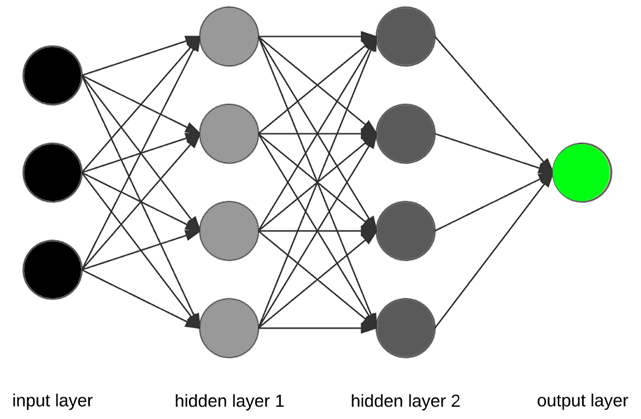
\includegraphics[scale=0.25]{images/fig-4.png}
\caption{Hidden Layer Between Input and Output Layers}
\label{fig:x Hidden Layer Between Input and Output Layers}
\end{figure}

\section{Dataset, Libraries, and Tools}
As our data are mostly direct fundus images from LAG-Dataset[24]. CNN is being used in this thesis for image classification, as it is a type of model which processes data such as images. Also, it automatically understands low-to high-level patterns of image classification. which helps us to extract higher representations for the image content.

\vspace{5mm}
\begin{figure}[htbp]
\centering
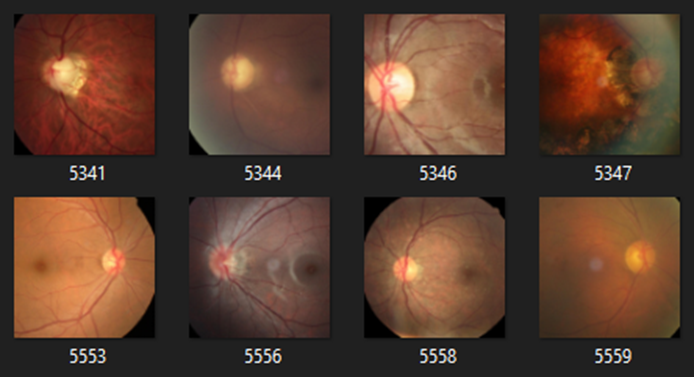
\includegraphics[scale=1]{images/fig-5.png}
\caption{Sample Data form LAG-Dataset}
\label{fig:x Sample Data form LAG-Dataset}
\end{figure}

This dataset contains 4250 images for \textbf{training}, 302 images for testing and 302 images for \textbf{validation}. All of these folders have two folders for glaucoma and non-glaucoma. The label for “glaucoma” is 1 and for “non-glaucoma” is 0.

\vspace{5mm}
\begin{table}[htbp]
\centering
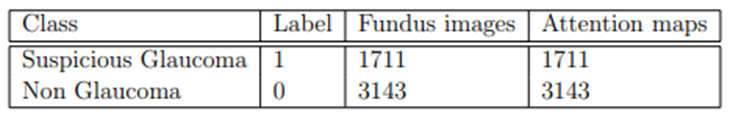
\includegraphics[scale=1]{images/fig-6.png}
\caption{\label{tab:Distribution of data with labels}Distribution of data with labels}

% \label{fig:x Distribution of data with labels }
\end{table}

In this study, we are going to use the \textbf{python} programming language. It is a high level OOP programming language that has a lot of amazing Machine learning libraries.

\vspace{5mm}
For this research we are using :

\begin{itemize}
    \item IDE (Google Colab & Jupyter Notebook)
    \item GPU (GTX 1660 super OC)
\end{itemize}

\newpage
Some of the Libraries that we are going to use are :

\vspace{5mm}
\textbf{TensorFlow}: TensorFlow is an end-to-end open-source platform for machine learning. It has a comprehensive, flexible ecosystem of tools, libraries, and communities [17].

\vspace{5mm}
\textbf{Keras}: Keras is the high-level API of TensorFlow 2: an approachable, highly-productive interface for solving machine learning problems [18]

\vspace{5mm}
\textbf{Matplotlib}: Matplotlib is a comprehensive library for creating static, animated, and interactive visualizations in Python.[25]

\vspace{5mm}
\textbf{Pandas}: Pandas is an open-source, BSD-licensed library providing high-performance, easy-to-use data structures, and data analysis tools for Python programming [26]

\vspace{5mm}
\textbf{Numpy}: NumPy offers comprehensive mathematical functions, random number generators, linear algebra routines, Fourier transforms, and more [19]

\vspace{5mm}
\textbf{Scikit-Learning}: Simple and efficient tools for predictive data analysis · Accessible to everybody, and reusable in various contexts · Built on NumPy, SciPy, and matplotlib [27]
 
\section{Architecture of the Proposed Model}
In deep learning, a convolutional neural network (CNN, or ConvNet) is a class of artificial neural networks, most commonly applied to analyze visual imagery[20].

\vspace{5mm}
In this study, a Transfer Learning approach is proposed. The data set's size and features provide a perfect environment for implementing a transfer learning approach, allowing a pre-trained CNN with all of its weights to be utilized to develop a new transfer learning model specialized to identifying Glaucoma with a high degree of accuracy.

\vspace{5mm}
\begin{figure}[hbt!]
\centering
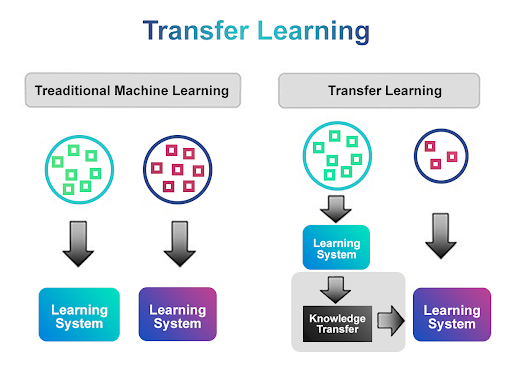
\includegraphics[scale=0.75]{images/fig-7.png}
\caption{Sample Data form LAG-Dataset}
\label{fig:x Sample Data form LAG-Dataset}
\end{figure}

\vspace{5mm}
We are going with the Fine-Tuning approach of Transfer Learning.

\vspace{5mm}
The CNN Models we are using are:

\begin{itemize}
    \item VGG-16
    \item InceptionV3
    \item VGG-19
    \item ResNet50
    \item DenseNet121
\end{itemize}

\subsection{VGG-16}
With 16-19 layers of weights and small convolution filters of (33), the VGG[29] Convolutional Neural Network built by Visual Geometry Group, the University of Oxford has achieved amazing results. ReLU non-linearly is used here for hidden layers.

\vspace{5mm}
Here, we used the Keras implementation of the VGG16 model. We used the weights learned from the ImageNet dataset. We didn’t use the 3 fully connected layers at the top of the network. Input shape of the images is 224 x 224 and there are 3 channels. First, we flattened the model outputs. We used the “ReLU” activation function for the layers. For predictions, we used the “Softmax” activation function. 

\vspace{5mm}
In figure 5.4 we can visualize the architecture of the VGG-16  model.

\vspace{5mm}
\begin{figure}[hbt!]
\centering
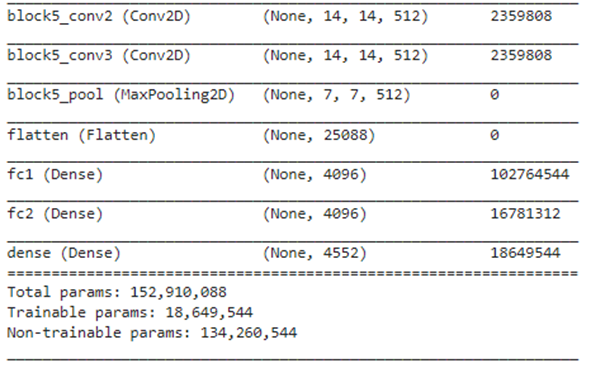
\includegraphics[scale=0.5]{images/fig-8.png}
\caption{Model Summary of VGG-16}
\label{fig:x Model Summary of VGG-16}
\end{figure}

\vspace{5mm}
In figure 5.5 we can visualize the architecture of the VGG-16  model.

\vspace{5mm}
\begin{figure}[hbt!]
\centering
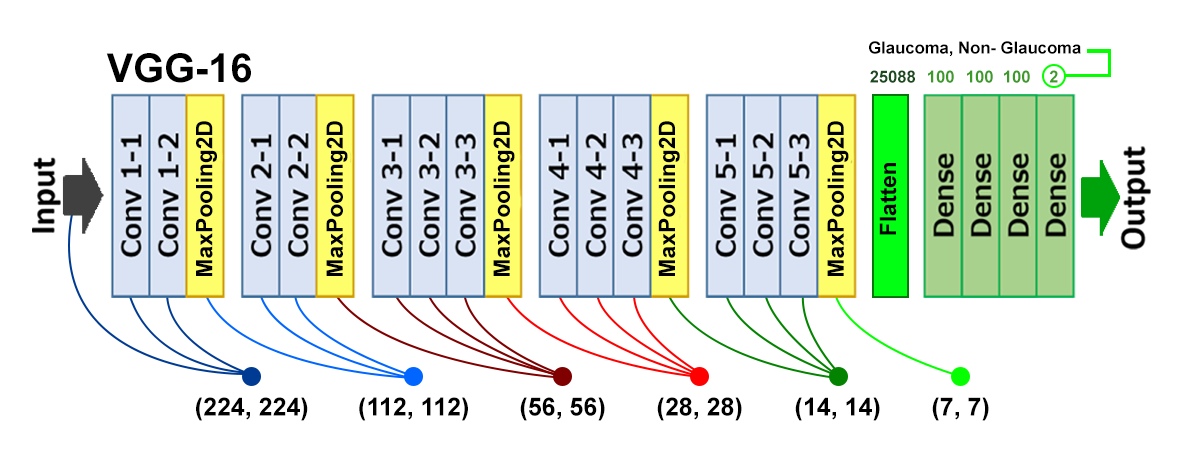
\includegraphics[scale=0.75]{images/Architecture of VGG-16.png}
\caption{Architecture of VGG-16}
\label{fig:x Architecture of VGG-16}
\end{figure}

\subsection{Inception V3}
The Inception [30] architecture is made up of several inception modules stacked on top of each other to form a deep neural network, where the inception modules provide the ability to operate them all in parallel and concatenate their outputs into a single output vector for input to the module afterward. 

\vspace{5mm}
Here we used Keras implementation of inceptionV3 model. We used the weights learned from the ImageNet dataset. We didn’t use the 3 fully connected layers at the top of the network. Input shape of the images is 224 x 224 and there are 3 channels. First, we flattened the model outputs. We used the “ReLU” activation function for the layers. For predictions, we used the “Softmax” activation function.

\vspace{5mm}
\begin{figure}[hbt!]
\centering
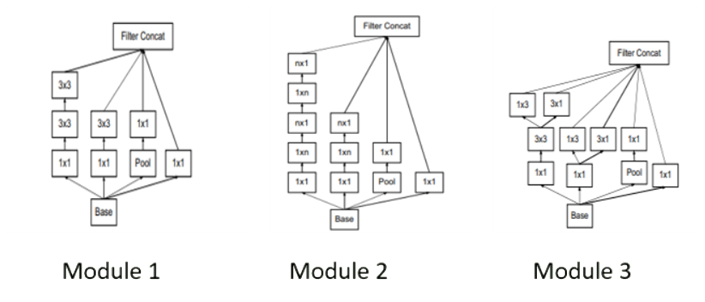
\includegraphics[scale=0.5]{images/fig-10.png}
\caption{The three inception modules}
\label{fig:x The three inception modules}
\end{figure}

\vspace{5mm}
In our proposed transfer learning model, we use InceptionV3, a new form of the inception architecture. Table 5.2 depicts the InceptionV3 network architecture. Each module's output size is the next module's input size. 

\begin{table}[hbt!]
\centering
\begin{tabular}{|c | c | c|}
\hline
Type & patch size & input size\\
\hline
conv & 3 x 3/2 & 224 x 224 x 3\\
\hline
conv & 3 x 3/1 & 149 x 149 x 32\\
\hline
conv padded & 3x3 / 1 & 147 x 147 x 32\\
\hline
pool & 3x3/2 & 147 x 147 x 64\\
\hline
conv & 3×3/1 & 73 × 73 × 64\\
\hline
conv & 3×3/2 & 71 × 71 × 80\\
\hline
conv & 3×3/1 & 35 × 35 × 192\\
\hline
3×Inception & module 1 & 35 × 35 × 288\\
\hline
5×Inception & module 2 & 17 × 17 × 768\\
\hline
2×Inception & module 3 & 8 × 8 × 1280\\
\hline
pool & 8×8 & 8 ×8 × 2048\\
\hline
linear & logits & 1 ×1 × 2048\\
\hline
softmax & classifier & 1 ×1 × 1000\\
\hline

\end{tabular}
\caption{Outline of the InceptionV3 architecture}
\label{tab:Outline of the InceptionV3 architecture [31]
)}
\end{table}

In figure 5.7 we can visualize our model summary of InceptionV3.

\vspace{5mm}
\begin{figure}[hbt!]
\centering
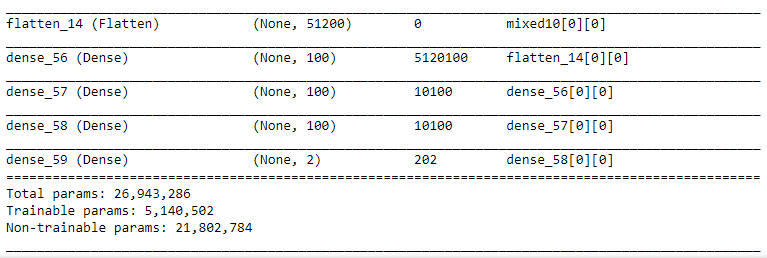
\includegraphics[scale=0.75]{images/fig-11.png}
\caption{Model Summary of InceptionV3}
\label{fig:x Model Summary of InceptionV3}
\end{figure}

\subsection{VGG-19}
VGG19 is a variant of the VGG model which in short consists of 19 layers (16 convolution layers, 3 fully connected layers, 5 MaxPool layers, and 1 SoftMax layer). [32] VGG19 has 19.6 billion Flops.

\vspace{5mm}
Here, we used the Keras implementation of the VGG19 model. We used the weights learned from the ImageNet dataset. We didn’t use the 3 fully connected layers at the top of the network. Input shape of the images is 224 x 224 and there are 3 channels. First, we flattened the model outputs. Then we performed batch normalization. We used a dropout rate of 0.5. We used the “ReLU” activation function for the layers.

\vspace{5mm}
For predictions, we used the “Softmax” activation function. For the Gradient Descent, we used the Adam optimizer with a learning rate of \(10^-5\). In Figure 5.8, Our model summary for VGG-19 is given.

\vspace{5mm}
\begin{figure}[hbt!]
\centering
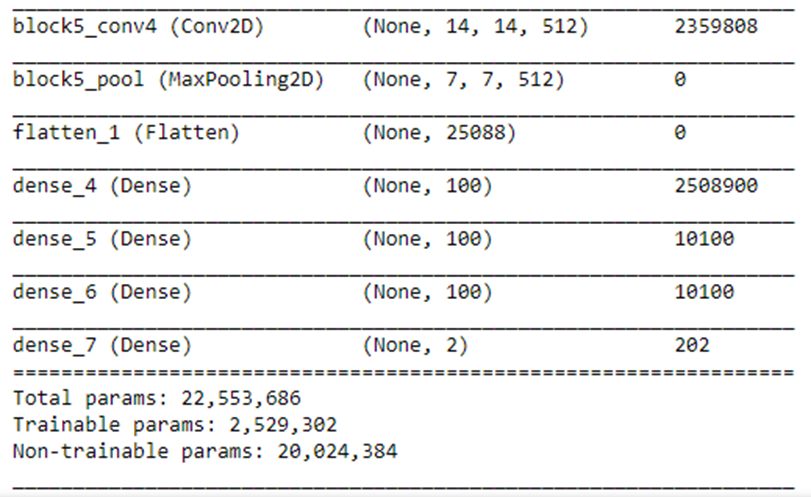
\includegraphics[scale=1]{images/fig-12.png}
\caption{Model Summary of VGG-19}
\label{fig:x Model Summary of VGG-19}
\end{figure}

\vspace{5mm}
\begin{figure}[hbt!]
\centering
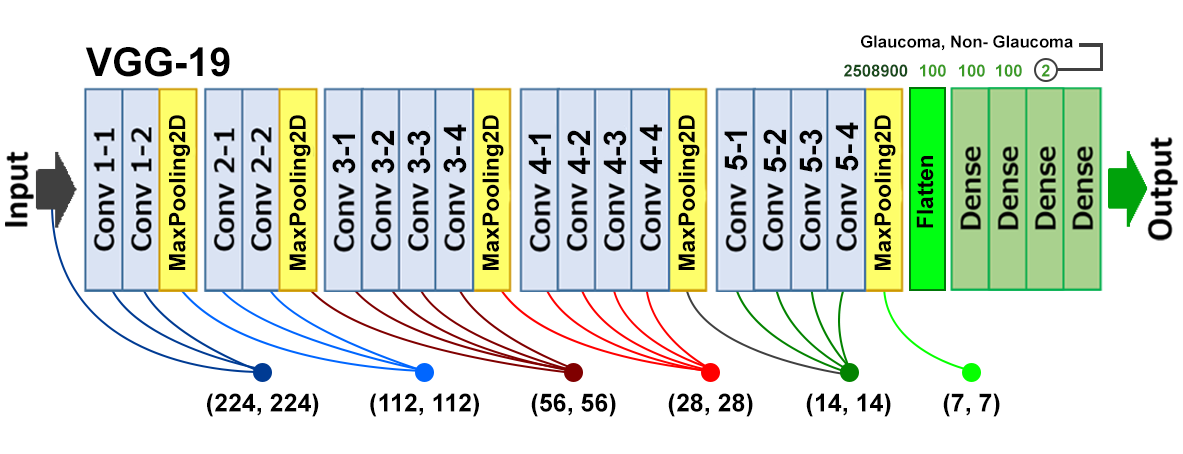
\includegraphics[scale=0.75]{images/Architecture of VGG-19.png}
\caption{Architecture of VGG-19}
\label{fig:x Architecture of VGG-19}
\end{figure}

\subsection{ResNet50}
ResNet50 is a version of the ResNet model which has 48 convolution layers and 1 MaxPool layer and 1 average pool layer. Moreover, it has 3.8 x \(10^9\) floating-point operations. ResNet50 plays an important role in the computer vision and deep learning world. It is mainly used for image recognition and is most commonly applied for analyzing visual imagery. Also, it is a pre-trained Deep Learning model for image classification of the Convolutional Neural Network (CNN). ResNet50 is mainly trained on a million images of 1000 categories from the ImageNet database and there are over 23 million trained parameters which will make it more suitable for image recognition. ResNet50 is deeper than any other network using residual connections.

\vspace{5mm}
Here, we used the Keras implementation of the ResNet50 Model. We used the weights learned from the ImageNet dataset. We didn’t use the 3 fully connected layers at the top of the network. Input shape of the images is 224 x 224 and there are 3 channels. First, we flattened the model outputs. Then we performed batch normalization. We used a dropout rate of 0.5. We used the “ReLU” activation function for the layers. Again we performed batch normalization and used a dropout rate of 0.5. For predictions, we used the “Softmax” activation function. 

\vspace{5mm}
\begin{figure}[hbt!]
\centering
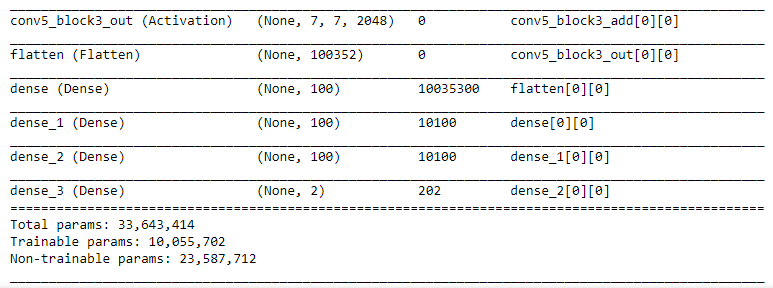
\includegraphics[scale=0.75]{images/ResNet50.PNG}
\caption{Model Summary of ResNet50}
\label{fig:x Model Summary of ResNet50}
\end{figure}

\subsection{DenseNet121}
Dense Convolutional Network which is DenseNet is an architecture that spotlights on making the profound learning networks go considerably more profound, and yet making them more proficient to prepare, by utilizing more limited associations between the layers [33]. DenseNet is very much like ResNet for certain key distinctions. For instance, ResNet utilizes an added substance strategy that combines the preceding layer with the future layer, while DenseNet links the result of the preceding layer with the future layer. This is done to empower the greatest data stream between the layers of the organization.

\vspace{5mm}
Here, we used the Keras implementation of the DenseNet121 model . We used the weights learned from the ImageNet dataset. We didn’t use the 3 fully connected layers at the top of the network. Input shape of the images is 224 x 224 and there are 3 channels. We performed  the 2D Global Average Pooling. Then we performed batch normalization. We used a dropout rate of 0.5. We used the “ReLU” activation function for the layers and again performed batch normalization and used a dropout rate of 0.5. For predictions, we used the “Softmax” activation function.

\vspace{5mm}
\begin{figure}[hbt!]
\centering
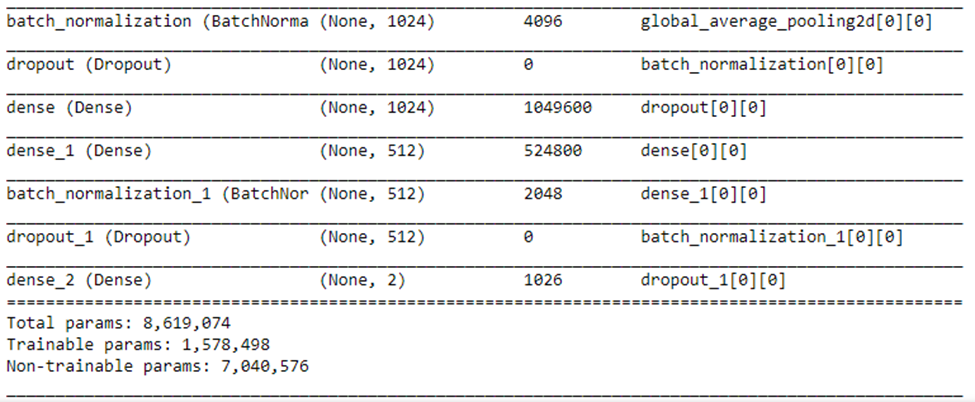
\includegraphics[scale=1]{images/fig-15.png}
\caption{Model Summary of DenseNet121}
\label{fig:x Model Summary of DenseNet121}
\end{figure}

\section{Fine Turing}
Fine-tuning is the process of fine-tuning or changing a model that has already been trained for one task to make it execute a second related task. A deep learning network that recognizes cars, for example, maybe fine-tuned to recognize trucks [25]. As proposed, we will be using Fine-tuning approach to detect Glaucoma from our dataset which will help to detect our wanted result in this study

\vspace{5mm}
\begin{figure}[hbt!]
\centering
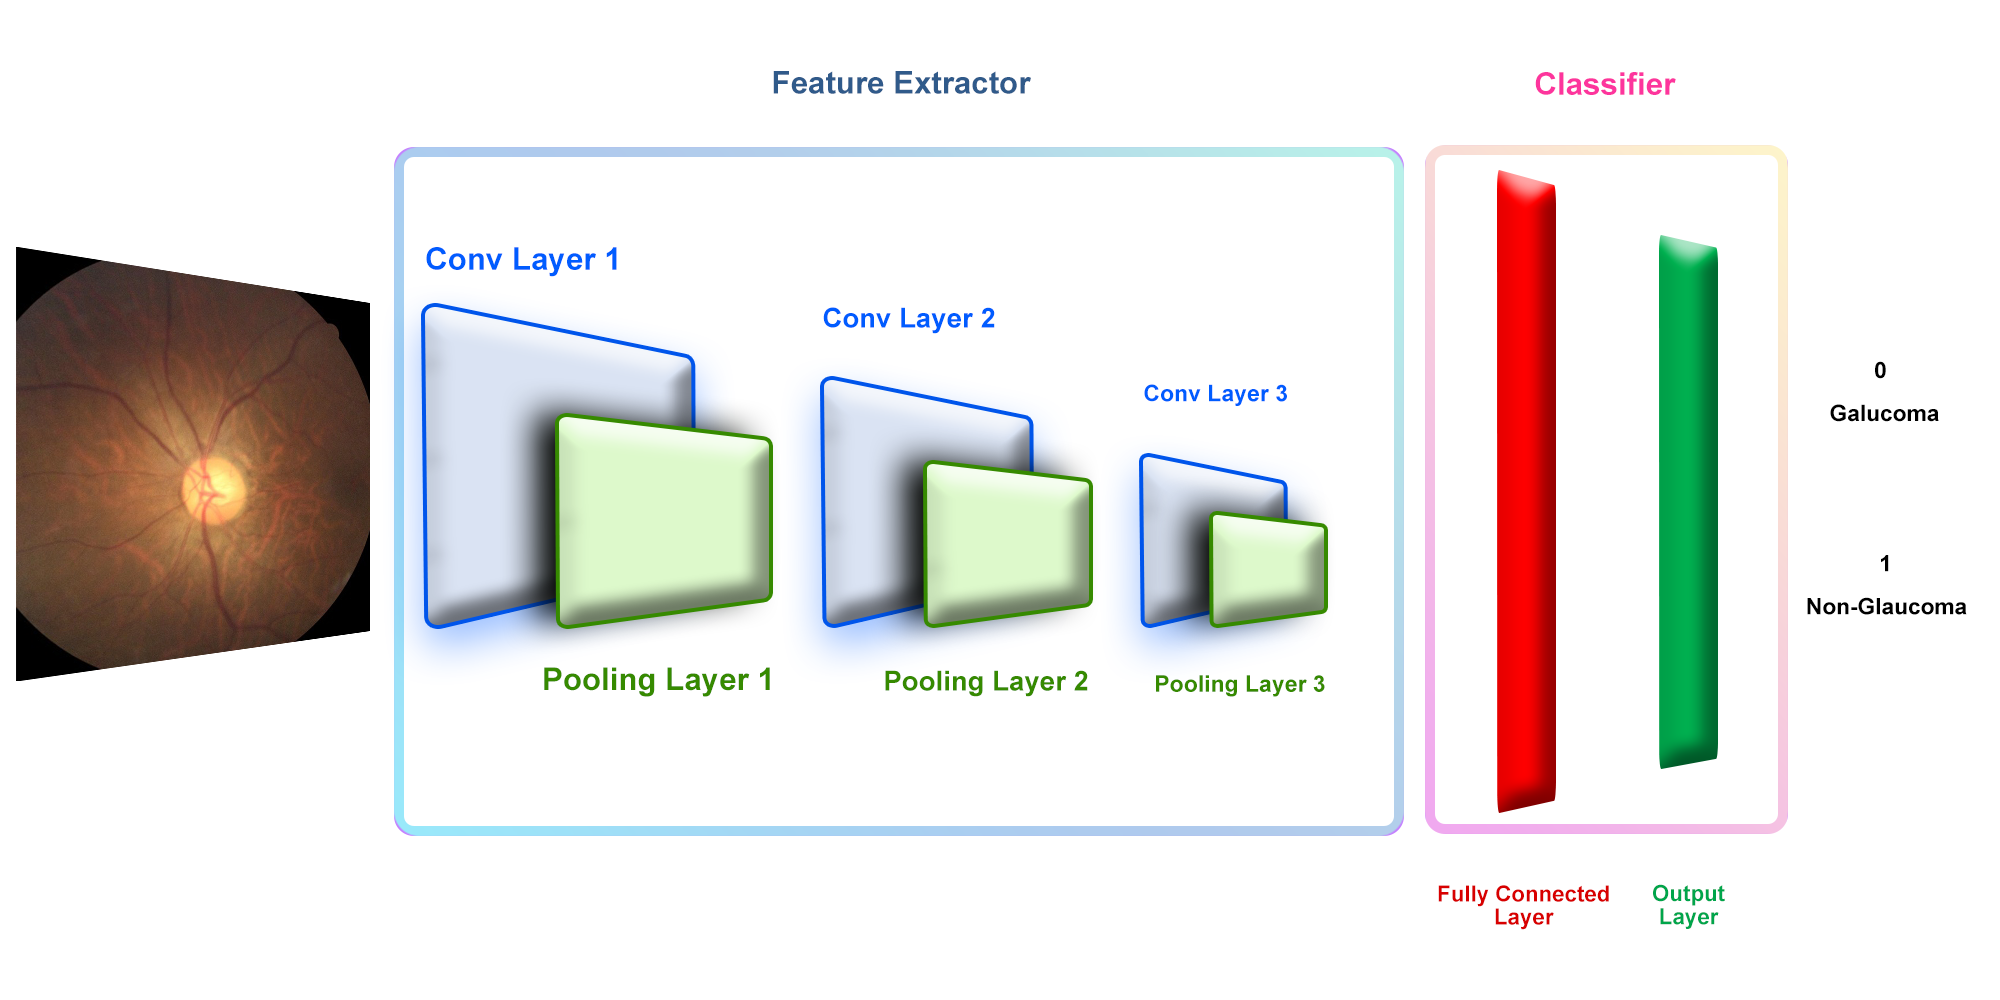
\includegraphics[scale=0.5]{images/Fine-tuning by keeping the feature extractor_s final layers trainable.png}
\caption{Fine-tuning by keeping the feature extractor's final layers trainable}
\label{fig:x Fine-tuning by keeping the feature extractor's final layers trainable}
\end{figure}

\newpage
\subsection{Segments of CNN}

\vspace{5mm}
The architecture of Convolutional Neural Networks is basically 3 types of layers.

\begin{itemize}
    \item Convolutional
    \item Pooling
    \item Fully Connected
\end{itemize}

\vspace{5mm}
\begin{figure}[hbt!]
\centering
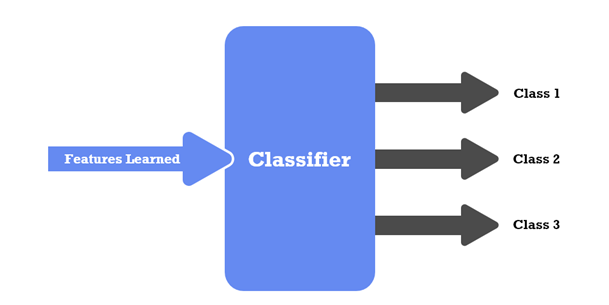
\includegraphics[scale=1]{images/fig-17.png}
\caption{CNN Classifier}
\label{fig:x CNN Classifier}
\end{figure}

And basically, all these layers do these operations as bellow:

\vspace{5mm}
\begin{itemize}
    \item Convolution operation
    \item Pooling operation
    \item Flattening
    \item Non-linear activation functions imply
    \item Optimization operation
\end{itemize}

\vspace{5mm}
\subsection{Convolutional Operation}


\vspace{5mm}
The convolutional layers, which are the fundamental building blocks of CNN, are responsible for convolution operations and produce feature maps that learn the features of the image taken as input by convolving appropriately learned filters or kernels with the input array or tensor, as shown in \textbf{figure 5.14}. A convolution layer, as shown in \textbf{figure 5.15}, has a number of feature maps that record new features and respond to feature hierarchy throughout the neural network, from the early layers to the distant edging layers.[29][34][30]

\newpage
\vspace{5mm}
\begin{figure}[hbt!]
\centering
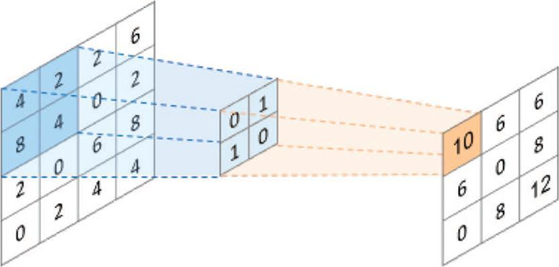
\includegraphics[scale=1]{images/fig-18.png}
\caption{On the input tensor, a kernel is applied, resulting in a feature map}
\label{fig:x On the input tensor, a kernel is applied, resulting in a feature map}
\end{figure}

\vspace{5mm}
\begin{figure}[hbt!]
\centering
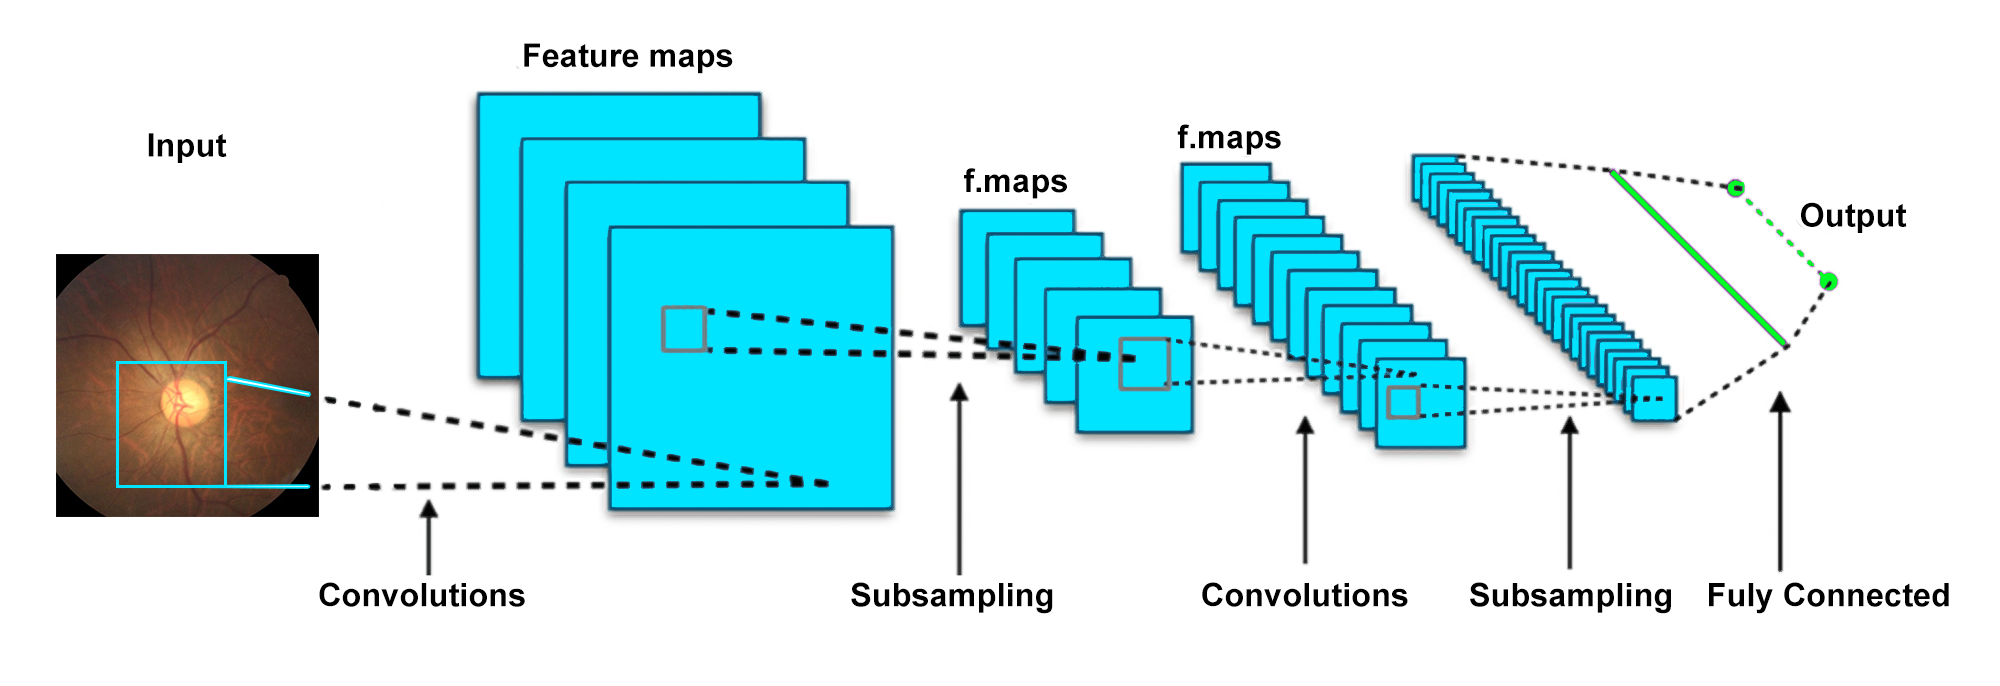
\includegraphics[scale=0.5]{images/planes shown are a feature map.png}
\caption{Planes shown are a feature map}
\label{fig:x Planes shown are a feature map}
\end{figure}

\subsection{Pooling Operation}

\vspace{5mm}
The feature maps are pooled in order to extract more features and minimize their dimension[30]. In general, the pooling operation is carried out as follows:

\vspace{5mm}
\begin{figure}[hbt!]
\centering
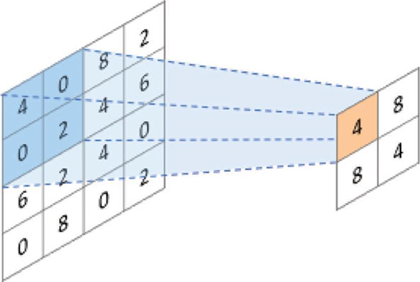
\includegraphics[scale=1]{images/fig-20.png}
\caption{Pooling Operation}
\label{fig:x Pooling Operation}
\end{figure}

\vspace{5mm}
\begin{itemize}
    \item \textbf{Max Pooling}: The maximum value of a patch of numbers from the feature map used as input is returned as an output. [30]
    \item \textbf{Average Pooling}: It produces the average value of a patch of numbers from the feature map that was used as input as an output. [34]
    \item \textbf{GlobalAveragePooling2D}:GlobalAveragePooling2D does something different. It applies average pooling on the spatial dimensions until each spatial dimension is one.
\end{itemize}

\vspace{5mm}
\begin{figure}[hbt!]
\centering
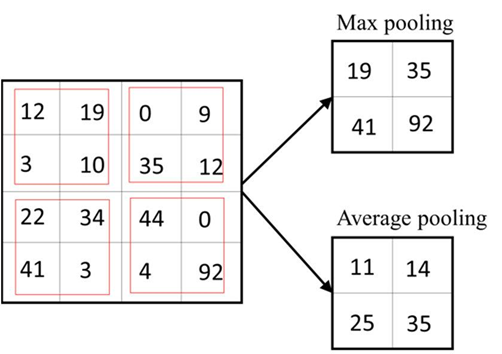
\includegraphics[scale=1]{images/fig-21.png}
\caption{Max and Average Pooling}
\label{fig:x Max and Average Pooling}
\end{figure}

\vspace{5mm}
\subsection{Flattening Layers}

\vspace{5mm}
Flattening is the process of turning data into a one-dimensional array for use in the following layer. To produce a single lengthy feature vector, we flatten the output of the convolutional layers. It's also linked to the final classification model, which is referred to as a fully-connected layer. [35]

\vspace{5mm}
\begin{figure}[hbt!]
\centering
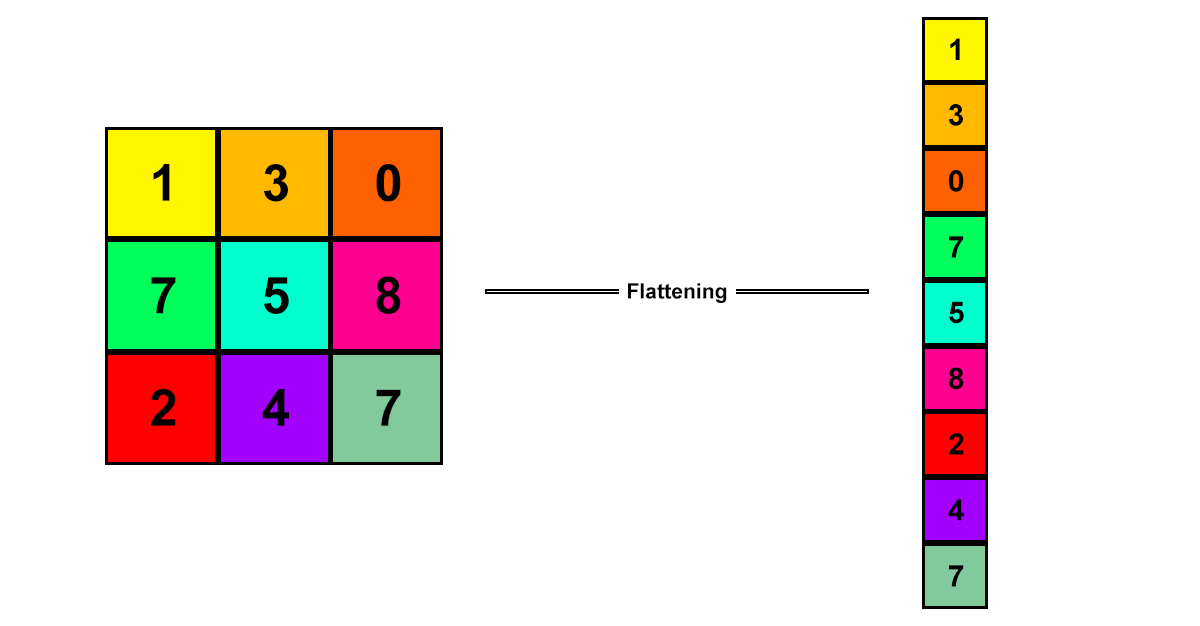
\includegraphics[scale=0.5]{images/Pooling Matrix to Flattening..png}
\caption{Pooling Matrix to Flattening.}
\label{fig:x Pooling Matrix to Flattening}
\end{figure}

\vspace{5mm}
\subsection{Fully Connected Layers}

\vspace{5mm}
In a neural network, fully connected layers are those where all of the inputs from one layer are connected to every activation unit of the subsequent layer. The last few layers in most standard machine learning models are fully connected layers that assemble the data collected by subsequent layers to produce the final output.[36]

\vspace{5mm}
\begin{figure}[hbt!]
\centering
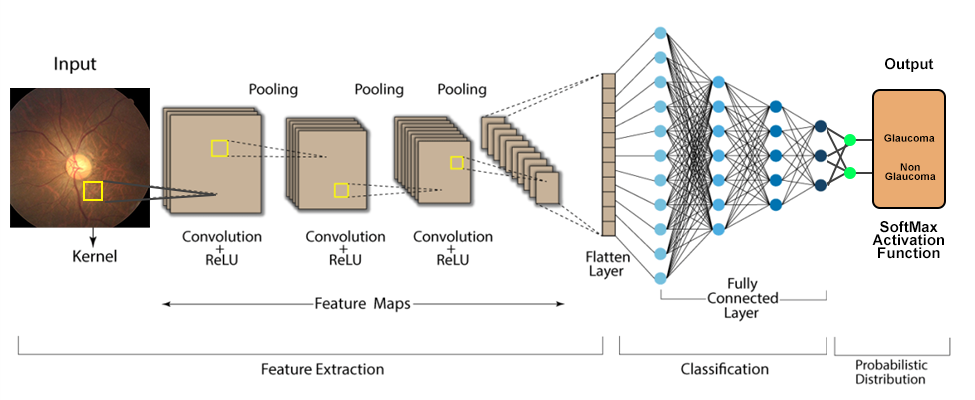
\includegraphics[scale=0.5]{images/Fully Connected CNN classifying between classes.png}
\caption{Fully Connected CNN classifying between classes}
\label{fig:x Fully Connected CNN classifying between classes}
\end{figure}

Fully connected layers or in other words dense layers take nonlinear activation functions, however, the final output layer of the fully connected layers take Softmax activation.

\vspace{5mm}
We are also going to use sigmoid and ReLU in both VGG-16 and InceptionV3.

\vspace{5mm}
\subsection{Batch Normalization}

\vspace{5mm}
While feeding input to Neural Networks, we do Batch Normalization because it makes the training faster and handles internal covariate shift. Again Normalizing the input for a similar range of values can speed up the learning. Because Batch Normalization normalizes the outputs of the activation functions in every layer of the neural network, not just in the inputs. In their original paper, Sergey et al. [37] claim that Batch Normalization reduces the internal covariate shift of the network.

\vspace{5mm}
\subsection{Dropout}

\vspace{5mm}
Adulteration of training information misleadingly regulates to overfit through dropout and other characteristical noise systems. Dropout holds out a kind of versatile regularization for summed up straight models [38]. Moreover, Dropout is a normal stochastic choice strategy in view of the neural organization [39]. This has the effect of making the layer look and be treated as a layer with a particular measure of hubs and availability to the past layer. Essentially, a particular perspective on the designed layer is directed with each update to a layer during preparing ...

\section{Analysis}
We have used VGG-16, VGG-19, DenseNet121, InceptionV3 and ResNet50 models for our study. Every model was compiled with Adam optimizer with the learning rate of 1e-5 in 50 epochs. 

These are the score(validation accuracy) our models - 

\vspace{5mm}
\begin{figure}[hbt!]
\centering
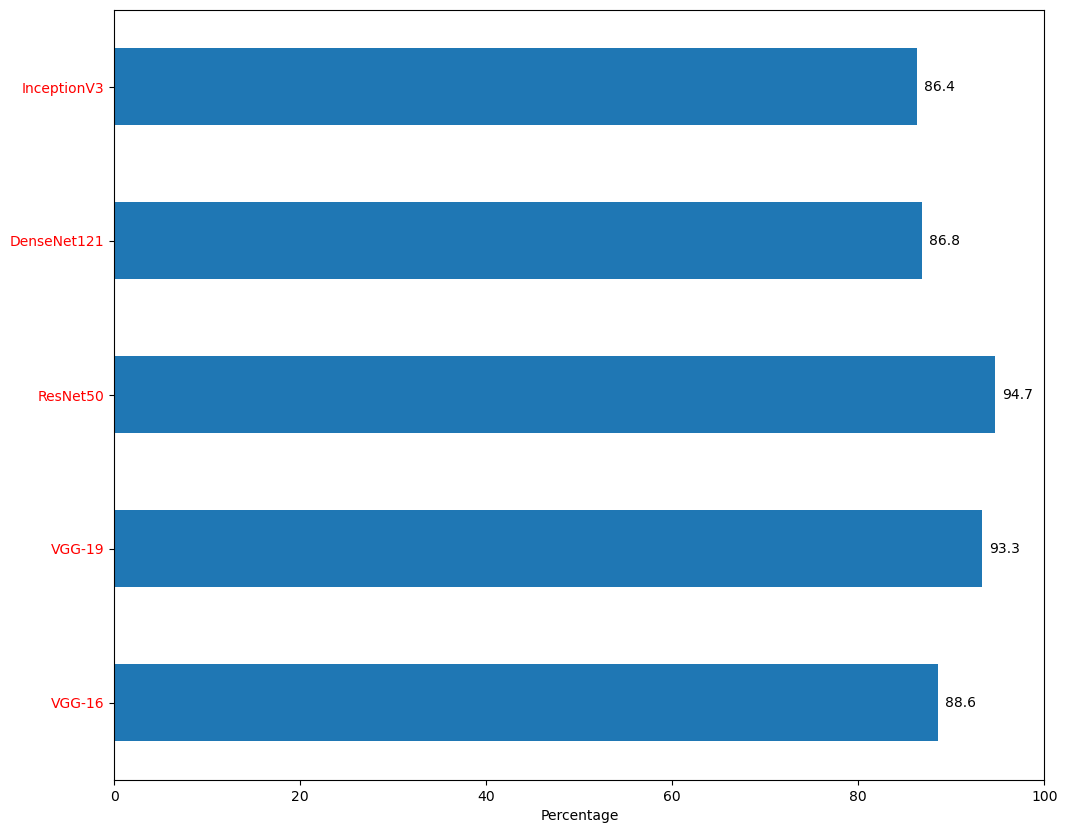
\includegraphics[scale=0.5]{images/fig-24.png}
\caption{Fully Connected CNN classifying between classes}
\label{fig:x Fully Connected CNN classifying between classes.}
\end{figure}

After 50 epochs, RestNet50 got the highest score among the other models with a validation accuracy of 94.7\%.

\vspace{5mm}
These are the Train and Test accuracy and loss graph for each model.

\newpage
\vspace{5mm}
Model Accuracy and Loss of VGG-16 -

\vspace{5mm}
\begin{figure}[hbt!]
\centering
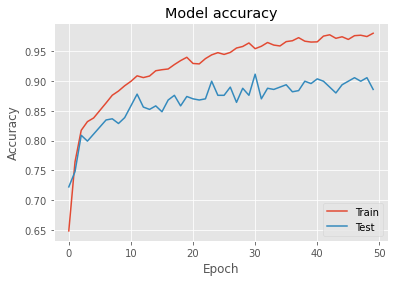
\includegraphics[scale=1]{images/fig-25.png}
\caption{VGG-16 Model Train and Test Accuracy}
\label{fig:x VGG-16 Model Train and Test Accuracy}
\end{figure}

\vspace{5mm}
\begin{figure}[hbt!]
\centering
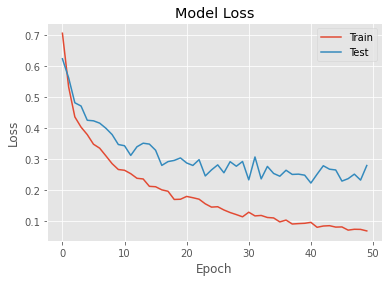
\includegraphics[scale=1]{images/fig-26.png}
\caption{VGG-16 Model Train and Test Loss}
\label{fig:x VGG-16 Model Train and Test Loss}
\end{figure}

\newpage
Model Accuracy and Loss of VGG-19 -

\vspace{5mm}
\begin{figure}[hbt!]
\centering
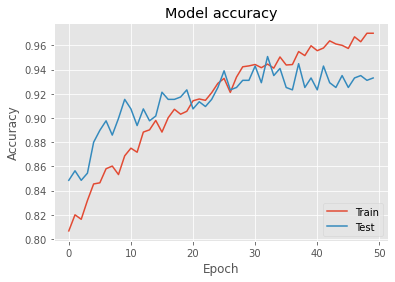
\includegraphics[scale=1]{images/fig-27.png}
\caption{VGG-19 Model Train and Test Accuracy}
\label{fig:x VGG-19 Model Train and Test Accuracy}
\end{figure}

\vspace{5mm}
\begin{figure}[hbt!]
\centering
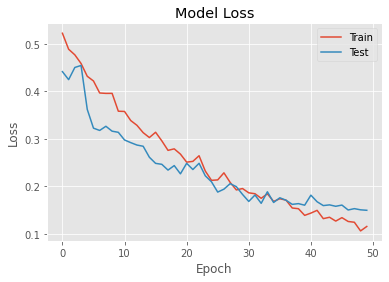
\includegraphics[scale=1]{images/fig-28.png}
\caption{VGG-19 Model Train and Test Loss}
\label{fig:x VGG-19 Model Train and Test Loss}
\end{figure}

\newpage
\vspace{5mm}
Model Accuracy and Loss of ResNet50 -
\vspace{5mm}
\begin{figure}[hbt!]
\centering
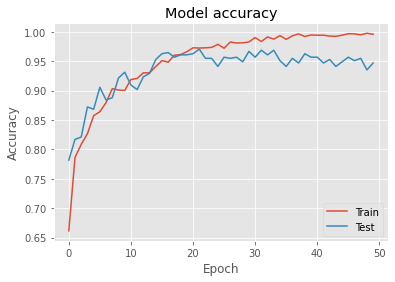
\includegraphics[scale=1]{images/fig-29.png}
\caption{ResNet50 Model Train and Test Accuracy}
\label{fig:x ResNet50 Model Train and Test Accuracy}
\end{figure}

\vspace{5mm}
\begin{figure}[hbt!]
\centering
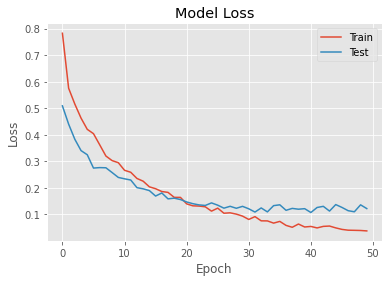
\includegraphics[scale=1]{images/fig-30.png}
\caption{ResNet50 Model Train and Test Loss}
\label{fig:x ResNet50 Model Train and Test Loss}
\end{figure}

\newpage
\vspace{5mm}
Model Accuracy and Loss of DenseNet121 -
\vspace{5mm}
\begin{figure}[hbt!]
\centering
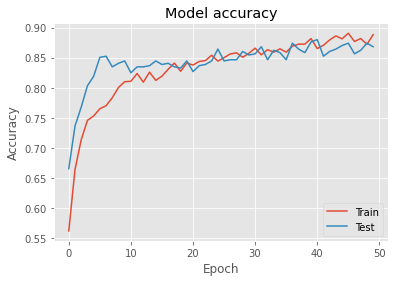
\includegraphics[scale=1]{images/fig-31.png}
\caption{DenseNet121 Model Train and Test Accuracy}
\label{fig:x DenseNet121 Model Train and Test Accuracy}
\end{figure}

\vspace{5mm}
\begin{figure}[hbt!]
\centering
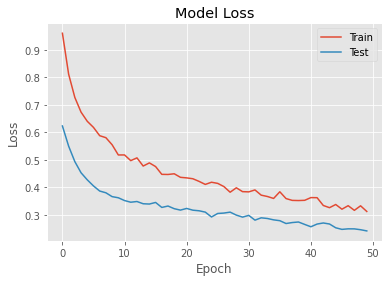
\includegraphics[scale=1]{images/fig-32.png}
\caption{DenseNet121 Model Train and Test Loss}
\label{fig:x DenseNet121 Model Train and Test Loss}
\end{figure}

\newpage
\vspace{5mm}
Model Accuracy and Loss of InceptionV3 -
\vspace{5mm}
\begin{figure}[hbt!]
\centering
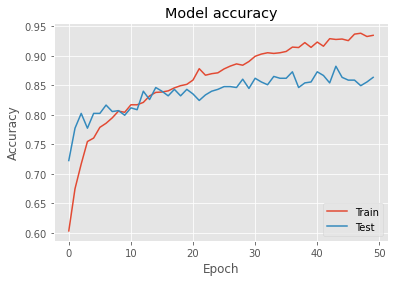
\includegraphics[scale=1]{images/fig-33.png}
\caption{InceptionV3 Model Train and Test Accuracy}
\label{fig:x InceptionV3 Model Train and Test Accuracy}
\end{figure}

\vspace{5mm}
\begin{figure}[hbt!]
\centering
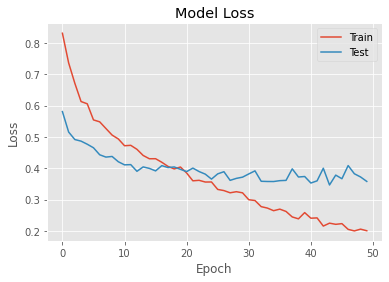
\includegraphics[scale=1]{images/fig-34.png}
\caption{InceptionV3 Model Train and Test Loss}
\label{fig:x InceptionV3 Model Train and Test Loss}
\end{figure}

The shape and dynamics of a learning curve can be used to diagnose the behavior of a machine learning model and in turn perhaps suggest the type of configuration changes that may be made to improve learning and/or performance.

\vspace{5mm}
There are three common dynamics that you are likely to observe in learning curves. And they are:

\begin{itemize}
    \item Underfit
    \item Overfit
    \item Good Fit
\end{itemize}

We know that smaller relative scores on the y-axis indicate more or better learning. 

\vspace{5mm}
\begin{figure}[hbt!]
\centering
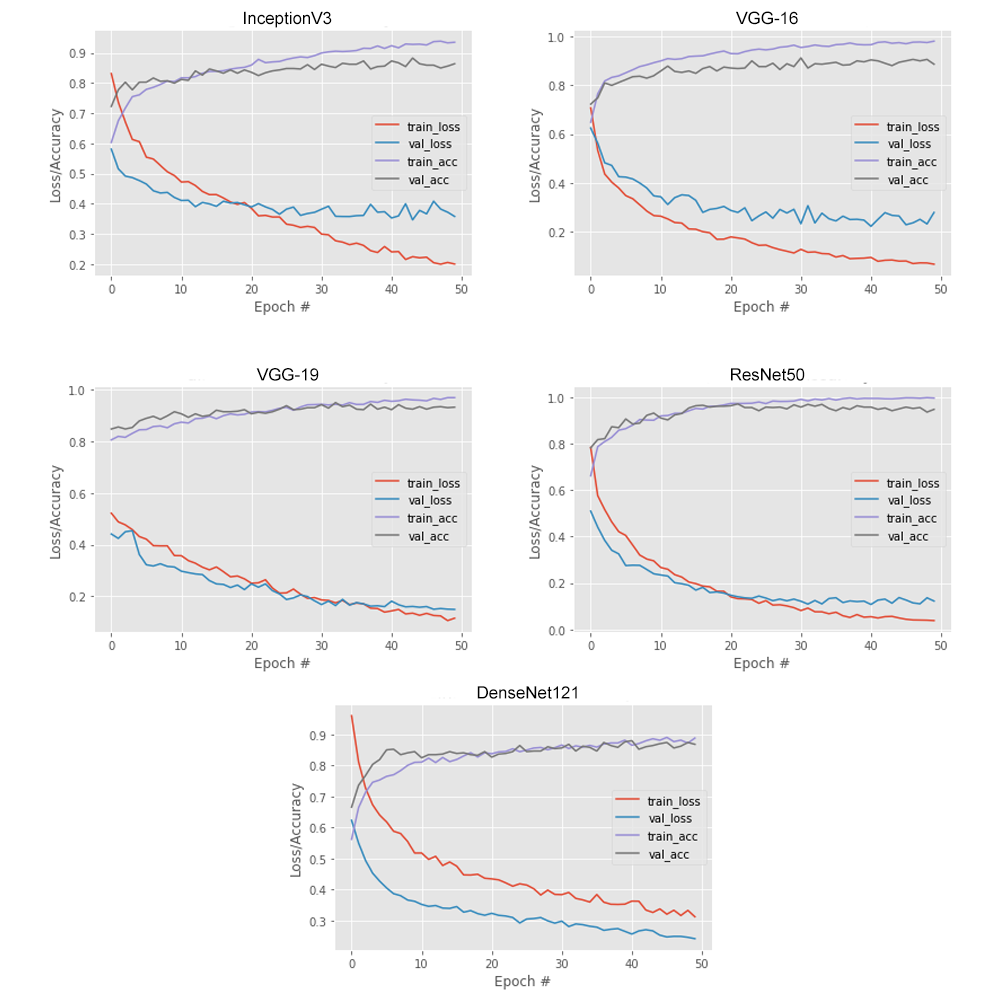
\includegraphics[scale=0.75]{images/fig-35.png}
\caption{All Model’s Train Test Accuracy and Loss Curve}
\label{fig:x All Model’s Train Test Accuracy and Loss Curve}
\end{figure}

\vspace{5mm}
Comparing All models' Accuracy and Loss graph together, we can see that VGG-19 and ResNet50 were the Good-Fit than the other models.

\vspace{5mm}
These are the Train sets, True and Predicted scores of classified and misclassified glaucoma and non-glaucoma results for each model based on the model’s train datasets prediction labels and the actual train labels. We have added a threshold of 0.5 for this train predicted visualization.

\vspace{5mm}
(the percentages are meaning the predicted train accuracy for the predicted labels calculated with the actual train labels)

\vspace{5mm}
\begin{figure}[hbt!]
\centering
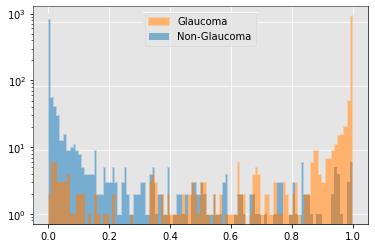
\includegraphics[scale=0.75]{images/fig-36.png}
\caption{True and Predicted Train scores of DenseNet121}
\label{fig:x True and Predicted Train scores of DenseNet121}
\end{figure}

% \centering
All  151 misclassified samples (93.83\%) 

Glaucoma  74 misclassified samples (93.95\%)

Non-Glaucoma  77 misclassified samples (93.71\%)

\vspace{5mm}
\begin{figure}[hbt!]
\centering
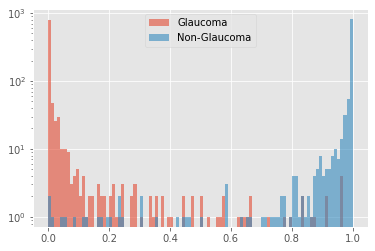
\includegraphics[scale=0.75]{images/fig-37.png}
\caption{True and Predicted Train scores of InceptionV3}
\label{fig:x True and Predicted Train scores of InceptionV3}
\end{figure}

% \centering
All   48 misclassified samples (97.65\%)

Glaucoma  22 misclassified samples (97.84\%)

Non-Glaucoma  26 misclassified samples (97.45\%)

\vspace{5mm}
\begin{figure}[hbt!]
\centering
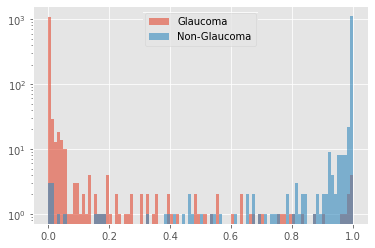
\includegraphics[scale=0.75]{images/fig-38.png}
\caption{True and Predicted Train scores of VGG-16}
\label{fig:x True and Predicted Train scores of VGG-16}
\end{figure}

\newpage
% \centering

All   47 misclassified samples (98.08\%)

Glaucoma  20 misclassified samples (98.37\%)

Non-Glaucoma  27 misclassified samples (97.79\%)

\vspace{5mm}
\begin{figure}[hbt!]
\centering
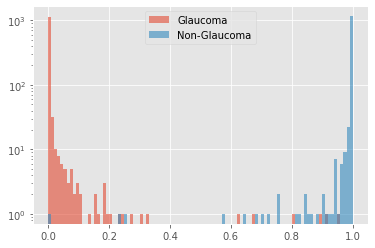
\includegraphics[scale=0.75]{images/fig-39.png}
\caption{True and Predicted Train scores of VGG-19}
\label{fig:x True and Predicted Train scores of VGG-19}
\end{figure}

All   17 misclassified samples (99.31\%)

Glaucoma  14 misclassified samples (98.86\%)

Non-Glaucoma   3 misclassified samples (99.75\%)

\vspace{5mm}
\begin{figure}[hbt!]
\centering
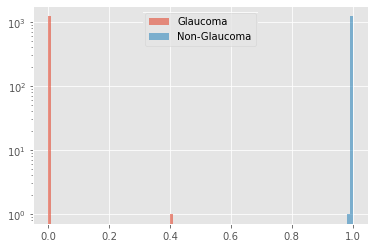
\includegraphics[scale=0.75]{images/fig-40.png}
\caption{True and Predicted Train scores of ResNet50}
\label{fig:x True and Predicted Train scores of ResNet50}
\end{figure}

\newpage

All    0 misclassified samples (100.00\%)

Glaucoma   0 misclassified samples (100.00\%)

Non-Glaucoma   0 misclassified samples (100.00\%)

\vspace{5mm}
Now, We have called the same function that we have used for the above Train predicted labels again with the same threshold of 0.5. But for now we have used the validation datasets prediction labels. And the results were - 

(the percentages are meaning the predicted test/validation accuracy for the predicted labels calculated with the actual test/validation labels)

\begin{table}[hbt!]
% \centering
\begin{tabular}{|c | c | c| c |}
\hline
Model & All misclassified & Glaucoma misclassified & Non-Glaucoma misclassified\\
\hline
DenseNet121 & 9 (86.76\%) & 4 (88.24\%) &  5 (85.29\%)\\
\hline
InceptionV3 & 24 (85.88\%) & 16 (81.18\%) & 8 (90.59\%)\\
\hline
VGG-16 & 8 (88.24\%) & 7 (79.41\%) & 1 (97.06\%)\\
\hline
VGG-19 & 4 (94.12\%) & 3 (91.18\%) & 1 (97.06\%)\\
\hline
ResNet50 & 3 (95.59\%) & 1 (97.06\%) & 2 (94.12\%)\\
\hline

\end{tabular}
\caption{True and Predicted Test scores of all Model}
\label{tab:True and Predicted Test scores of all Model}
\end{table}

\vspace{5mm}
Now we have taken a single predicted batch from each model’s prediction with the 0.5 threshold and plotted the misclassified glaucoma and non-glaucoma images, which we will use in Lime (XAI framework) to explain later.

\begin{table}[hbt!]
% \centering
\begin{tabular}{|c | c | c| c |}
\hline
Model & Batch & Glaucoma misclassified & Non-Glaucoma misclassified\\
\hline
DenseNet121 & 2 (32 in each) & 3 &  5\\
\hline
InceptionV3 & 2 (32 in each) & 2 & 7\\
\hline
VGG-16 & 2 (32 in each) & 2 & 3\\
\hline
VGG-19 & 2 (32 in each) & 1 & 4\\
\hline
ResNet50 & 2 (32 in each) & 0 & 3\\
\hline

\end{tabular}
\caption{True and Predicted Test scores of all Model}
\label{tab:True and Predicted Test scores of all Model}
\end{table}

\newpage
\vspace{5mm}
These are some of the misclassified images for all models with and undoing the existing preprocessing. Basically the model’s preprocessing for these images ruined their actual color and contrast.  Which led the model to predict wrong. By undoing the existing preprocessing we can see that for DesneNet121 the images got a little reddish and for other models, It got bluish.

\vspace{5mm}
\begin{figure}[hbt!]
\centering
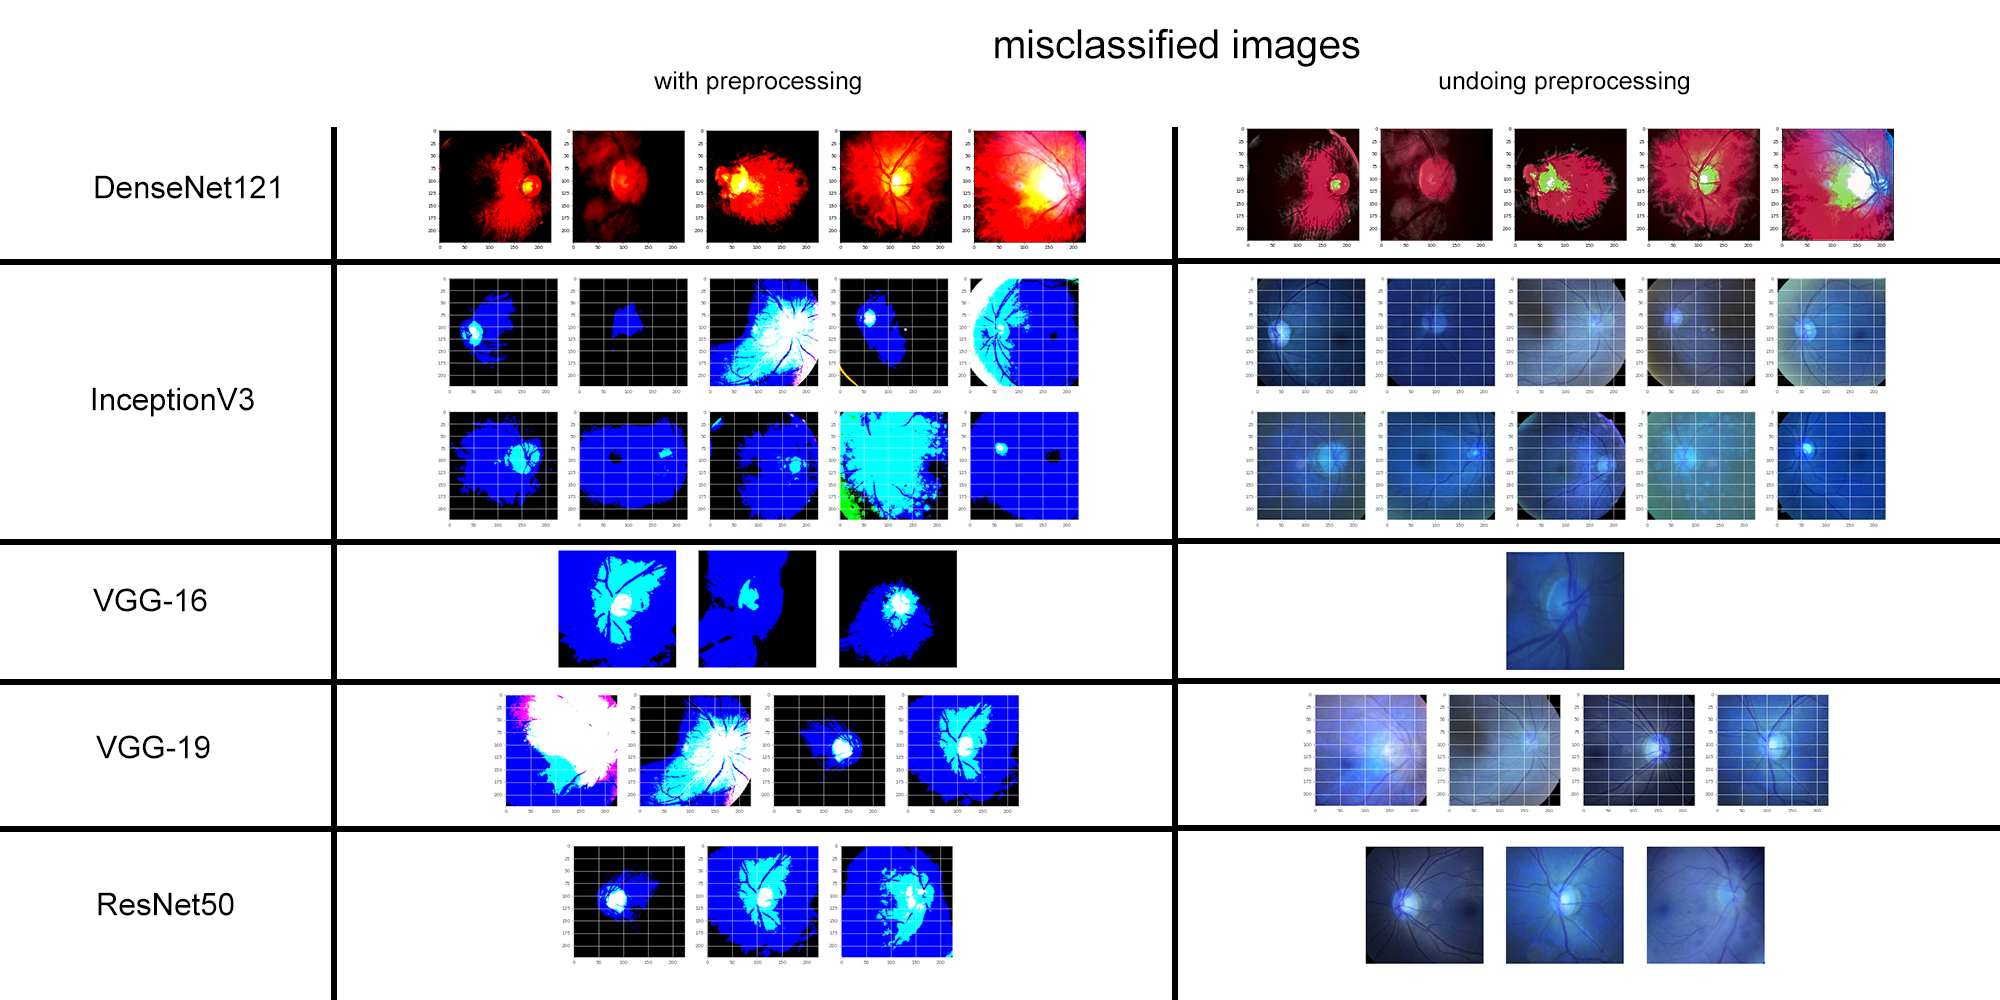
\includegraphics[scale=0.5]{images/fig-41.png}
\caption{True and Predicted Train scores of ResNet50}
\label{fig:x True and Predicted Train scores of ResNet50}
\end{figure}

\vspace{5mm}
Now we will show the explanation for these preprocessed and misclassified images using an XAI[40] framework, \textbf{LIME}. Then we will apply Lime again on a single predicted raw fundus -image directly from the test dataset (labelled) directory to see the difference between a correctly predicted fundus image[42] and wrong predicted fundus image.
Given below are the the misclassified image with preprocessing, Superpixels focused area and the model prediction explanation by Lime in DenseNet121 -

\vspace{5mm}
\begin{figure}[hbt!]
\centering
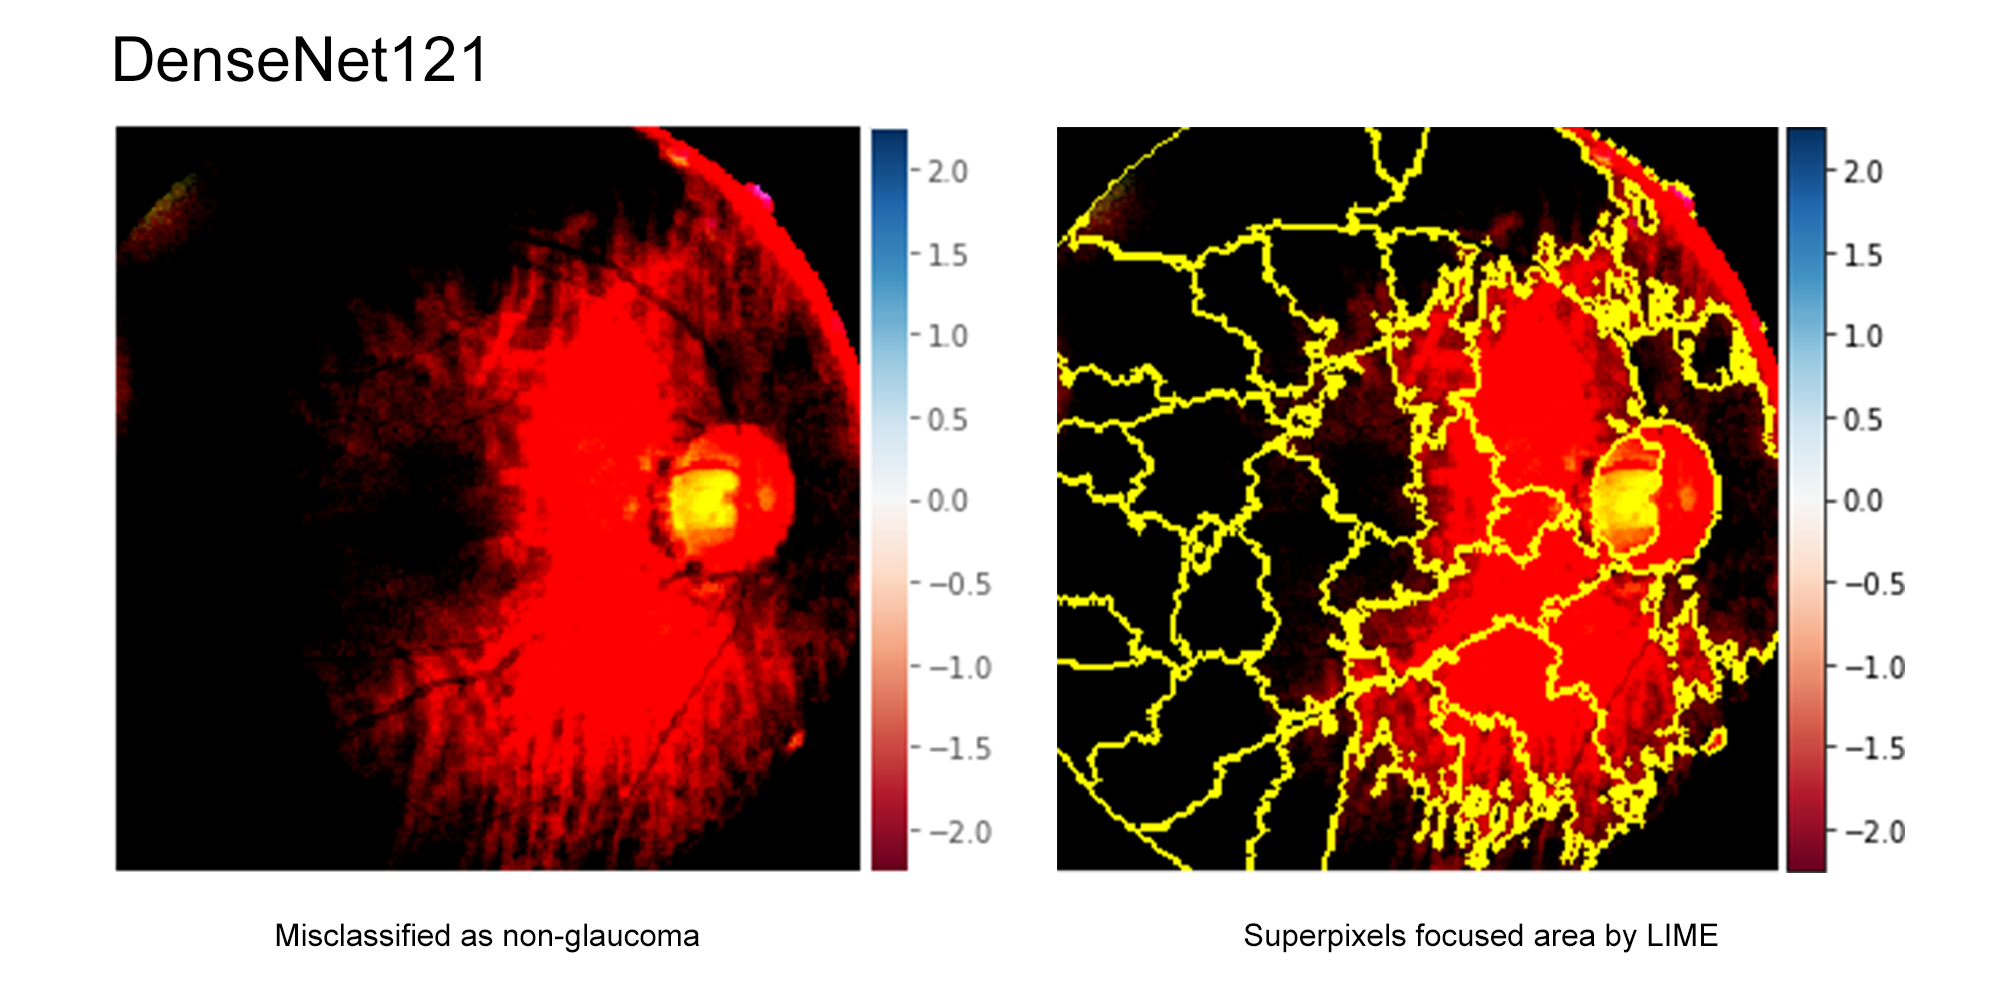
\includegraphics[scale=0.5]{images/fig-42.png}
\caption{Misclassified image with preprocessing and Superpixels focused area by Lime in DenseNet121}
\label{fig:x Misclassified image with preprocessing and Superpixels focused area by Lime in DenseNet121}
\end{figure}

\vspace{5mm}
\begin{figure}[hbt!]
\centering
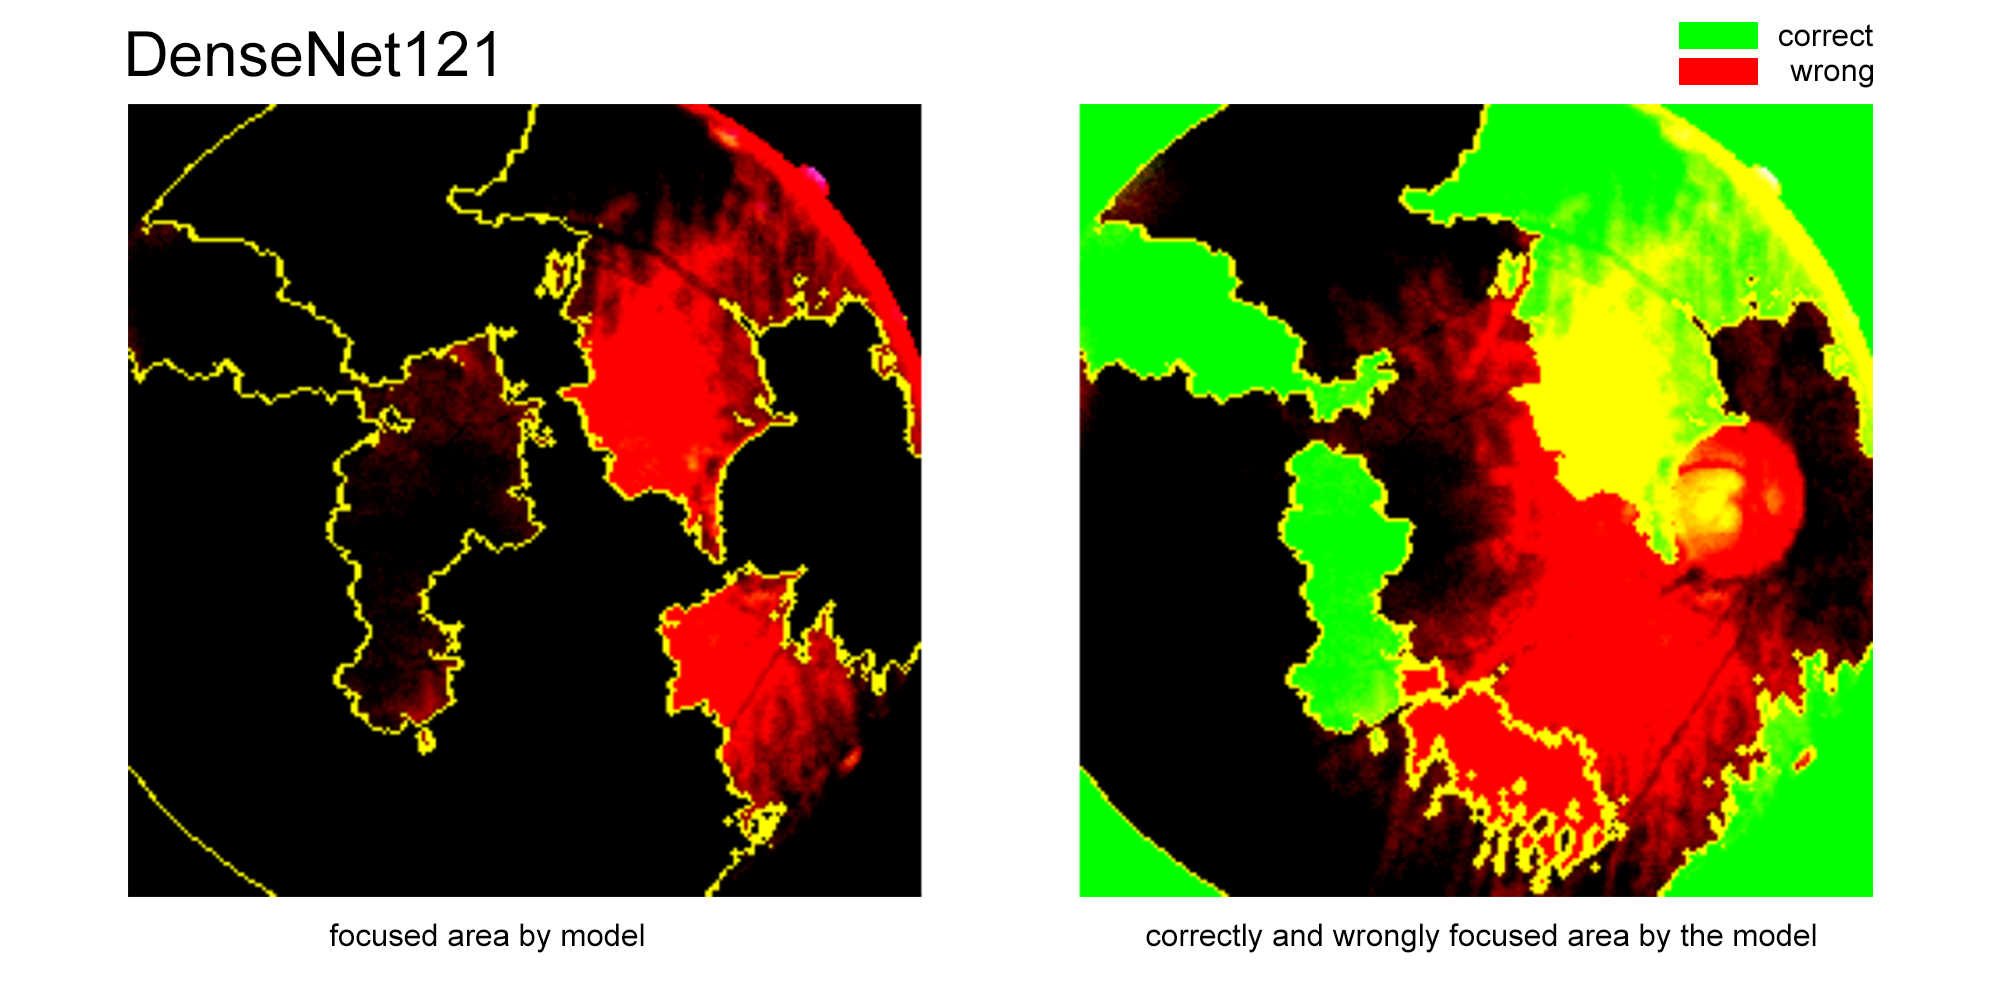
\includegraphics[scale=0.5]{images/fig-43.png}
\caption{Lime Explanation for DenseNet121}
\label{fig:x Lime Explanation for DenseNet121}
\end{figure}

\newpage
\vspace{5mm}
Given below are the the misclassified image with preprocessing, Superpixels focused area and the model prediction explanation by Lime in InceptionV3 -

\vspace{5mm}
\begin{figure}[hbt!]
\centering
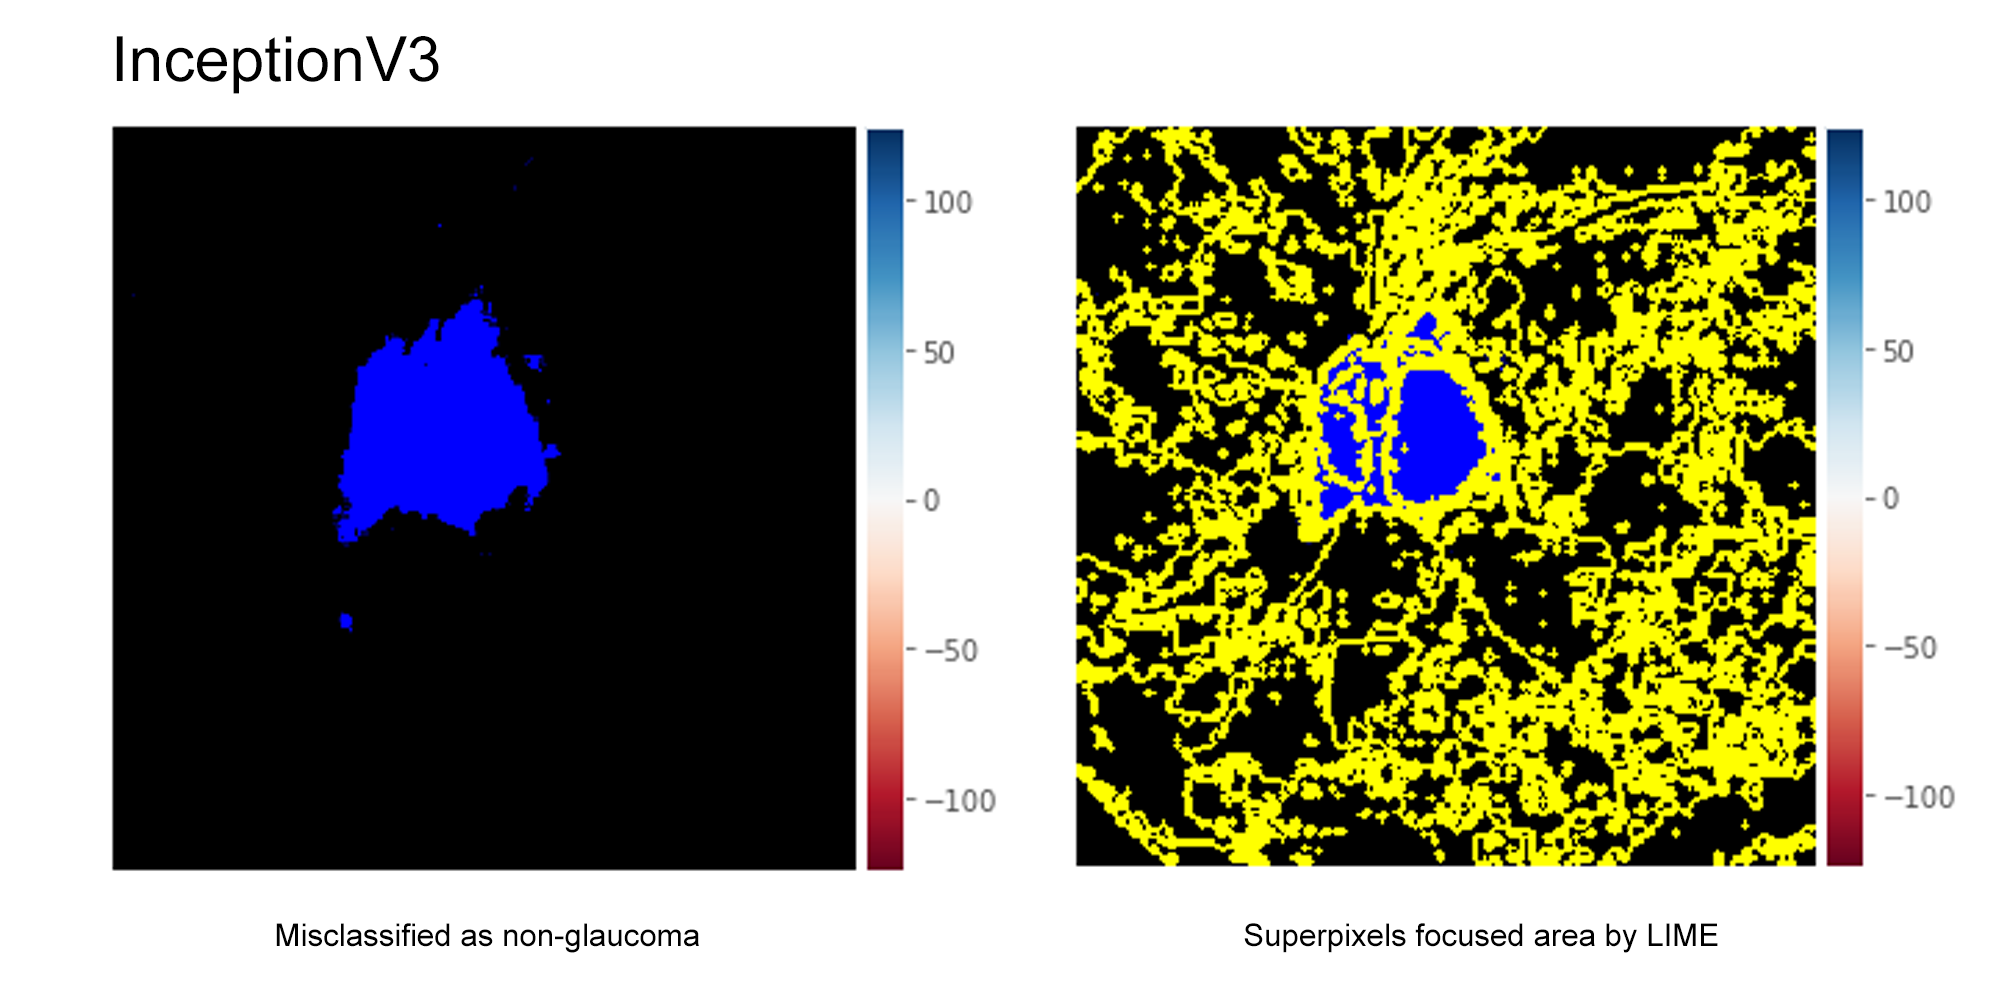
\includegraphics[scale=0.5]{images/fig-44.png}
\caption{Misclassified image with preprocessing and Superpixels focused area by Lime in InceptionV3
}
\label{fig:x Misclassified image with preprocessing and Superpixels focused area by Lime in InceptionV3
}
\end{figure}

\vspace{5mm}
\begin{figure}[hbt!]
\centering
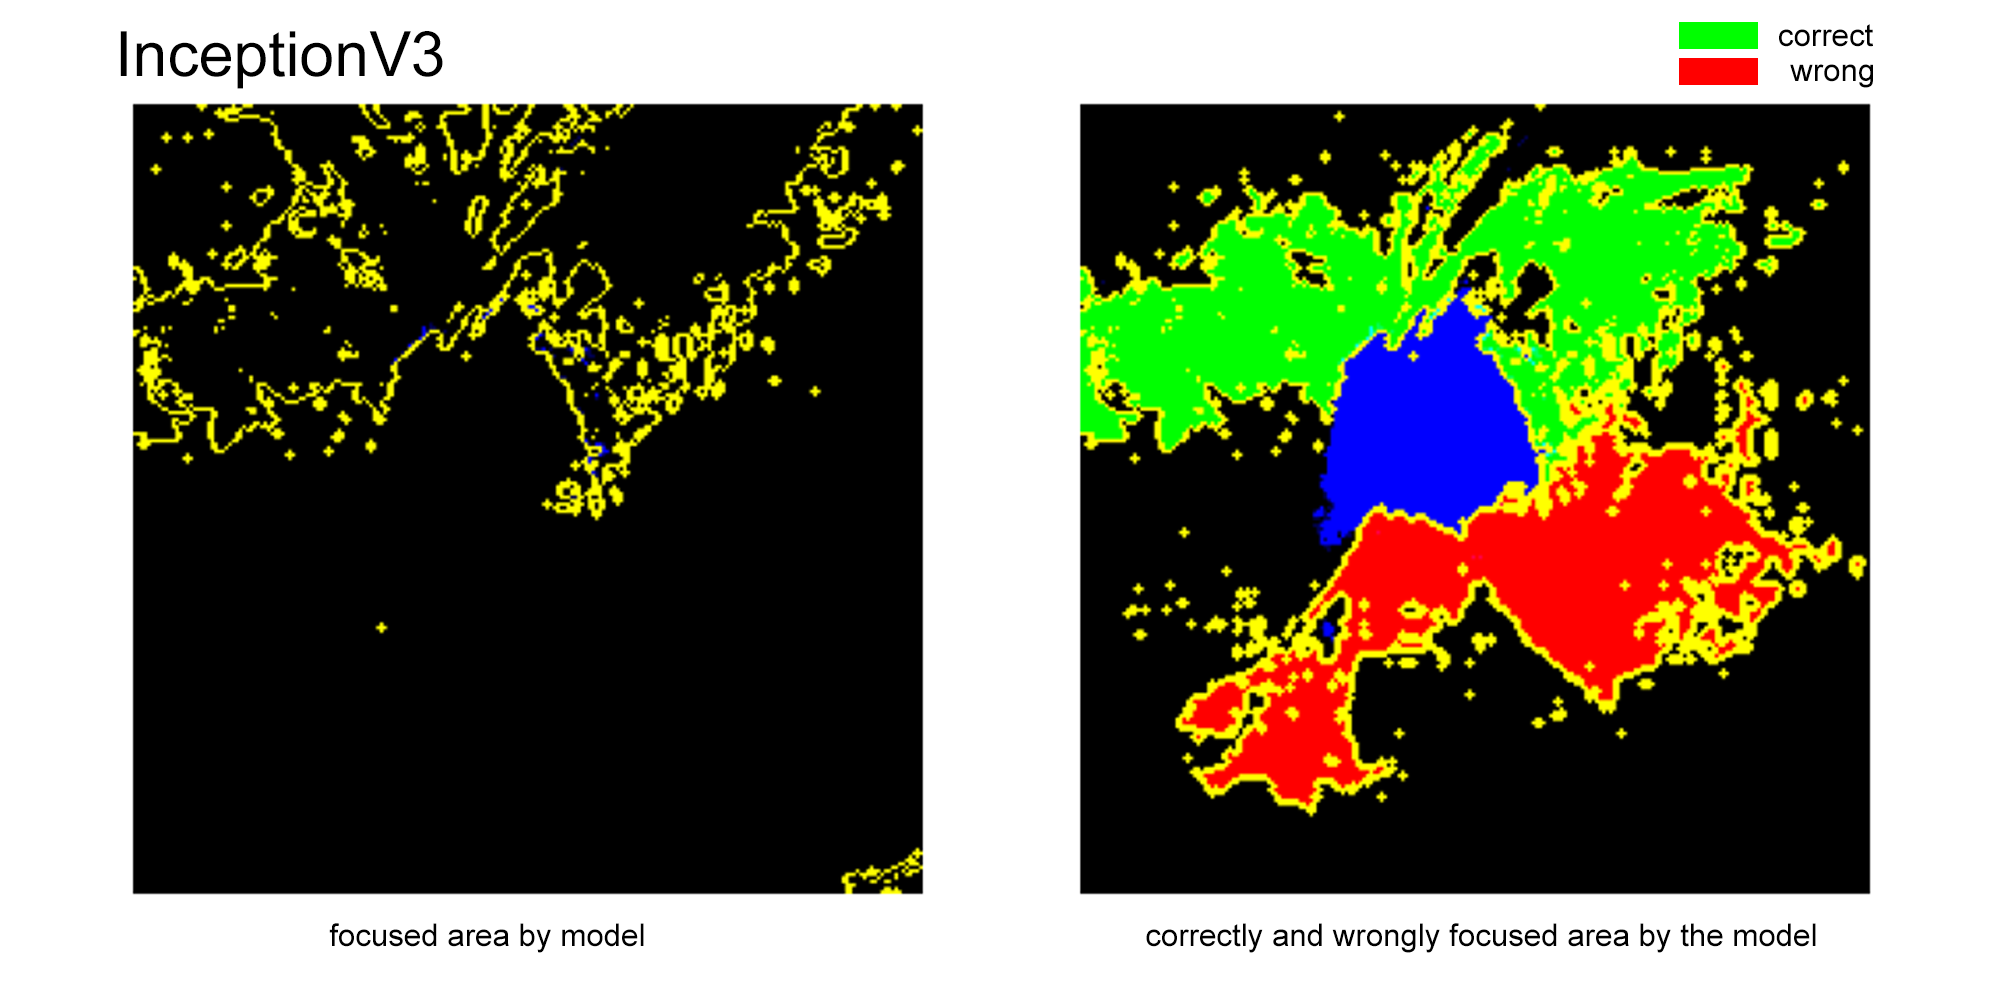
\includegraphics[scale=0.5]{images/fig-45.png}
\caption{Lime Explanation for InceptionV3}
\label{fig:x Lime Explanation for InceptionV3}
\end{figure}

\newpage
\vspace{5mm}
Given below are the the misclassified image with preprocessing, Superpixels focused area and the model prediction explanation by Lime in VGG-16 -

\vspace{5mm}
\begin{figure}[hbt!]
\centering
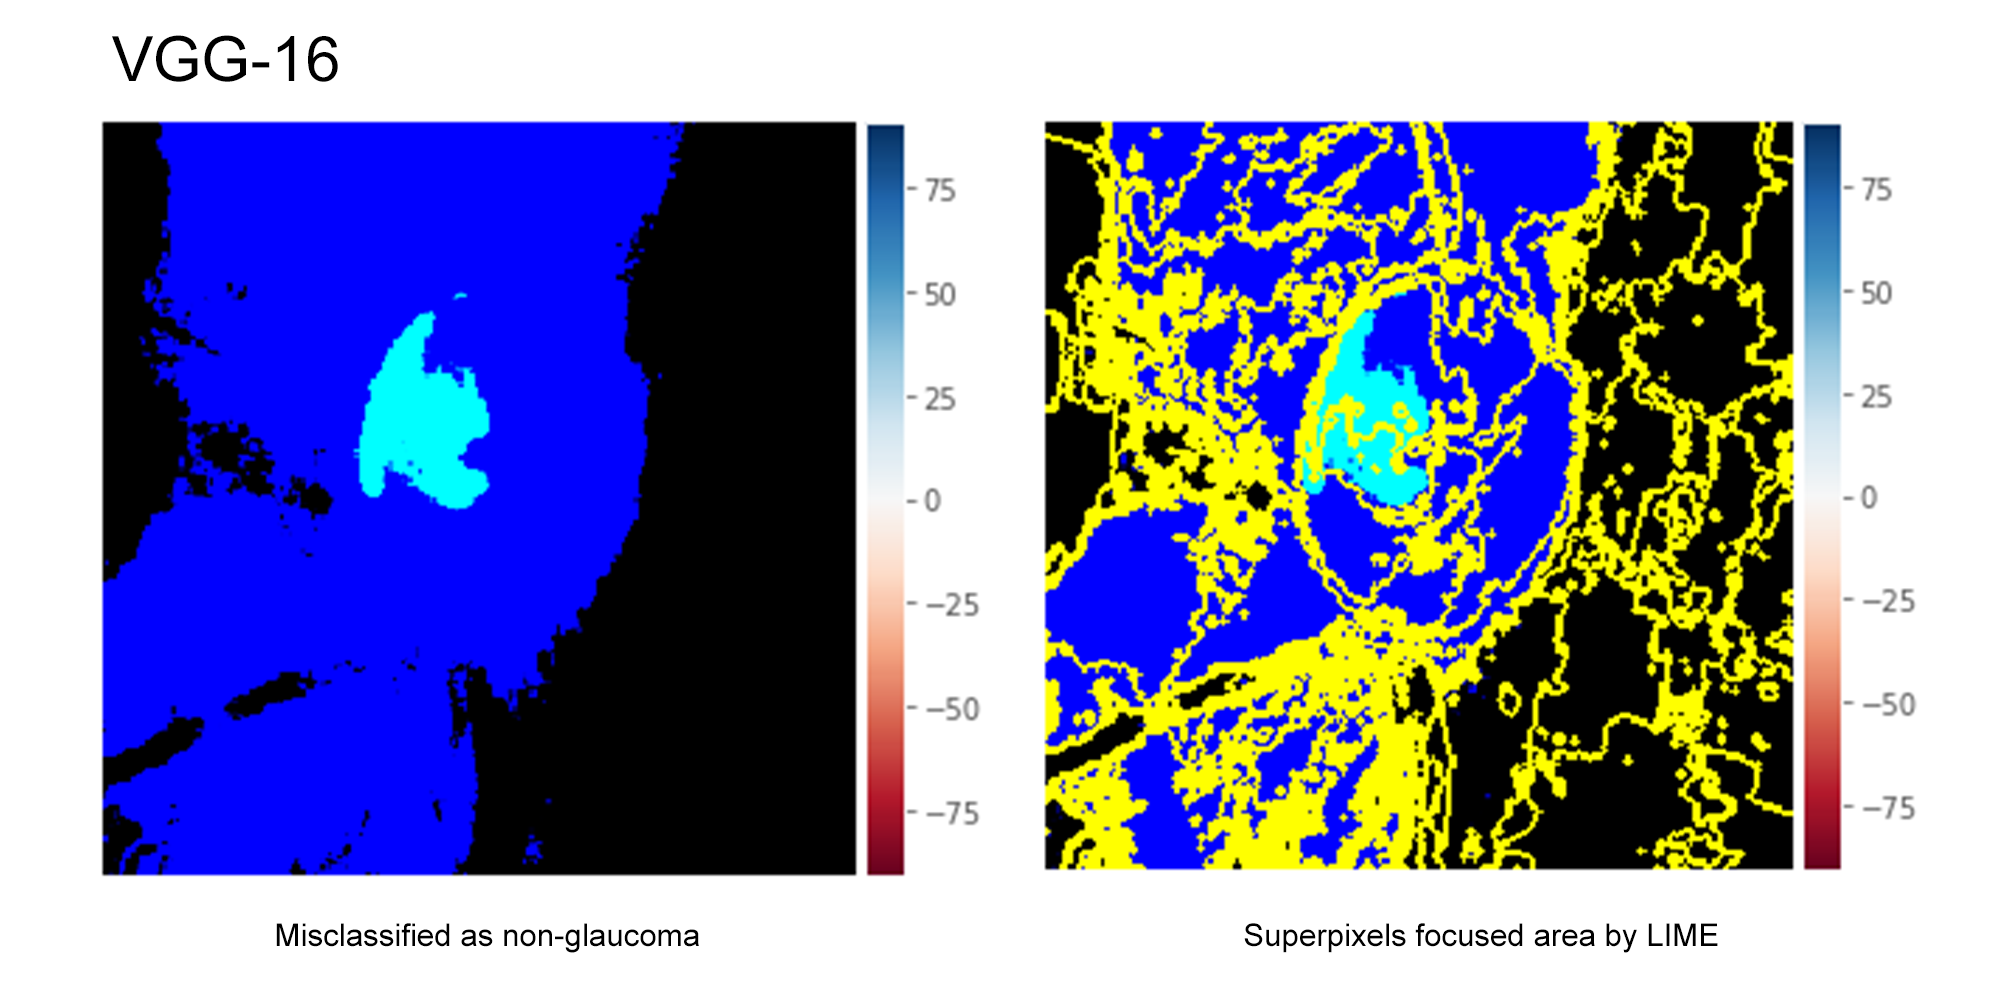
\includegraphics[scale=0.5]{images/fig-46.png}
\caption{Misclassified image with preprocessing and Superpixels focused area by Lime in VGG-16}
\label{fig:x Misclassified image with preprocessing and Superpixels focused area by Lime in VGG-16}
\end{figure}

\vspace{5mm}
\begin{figure}[hbt!]
\centering
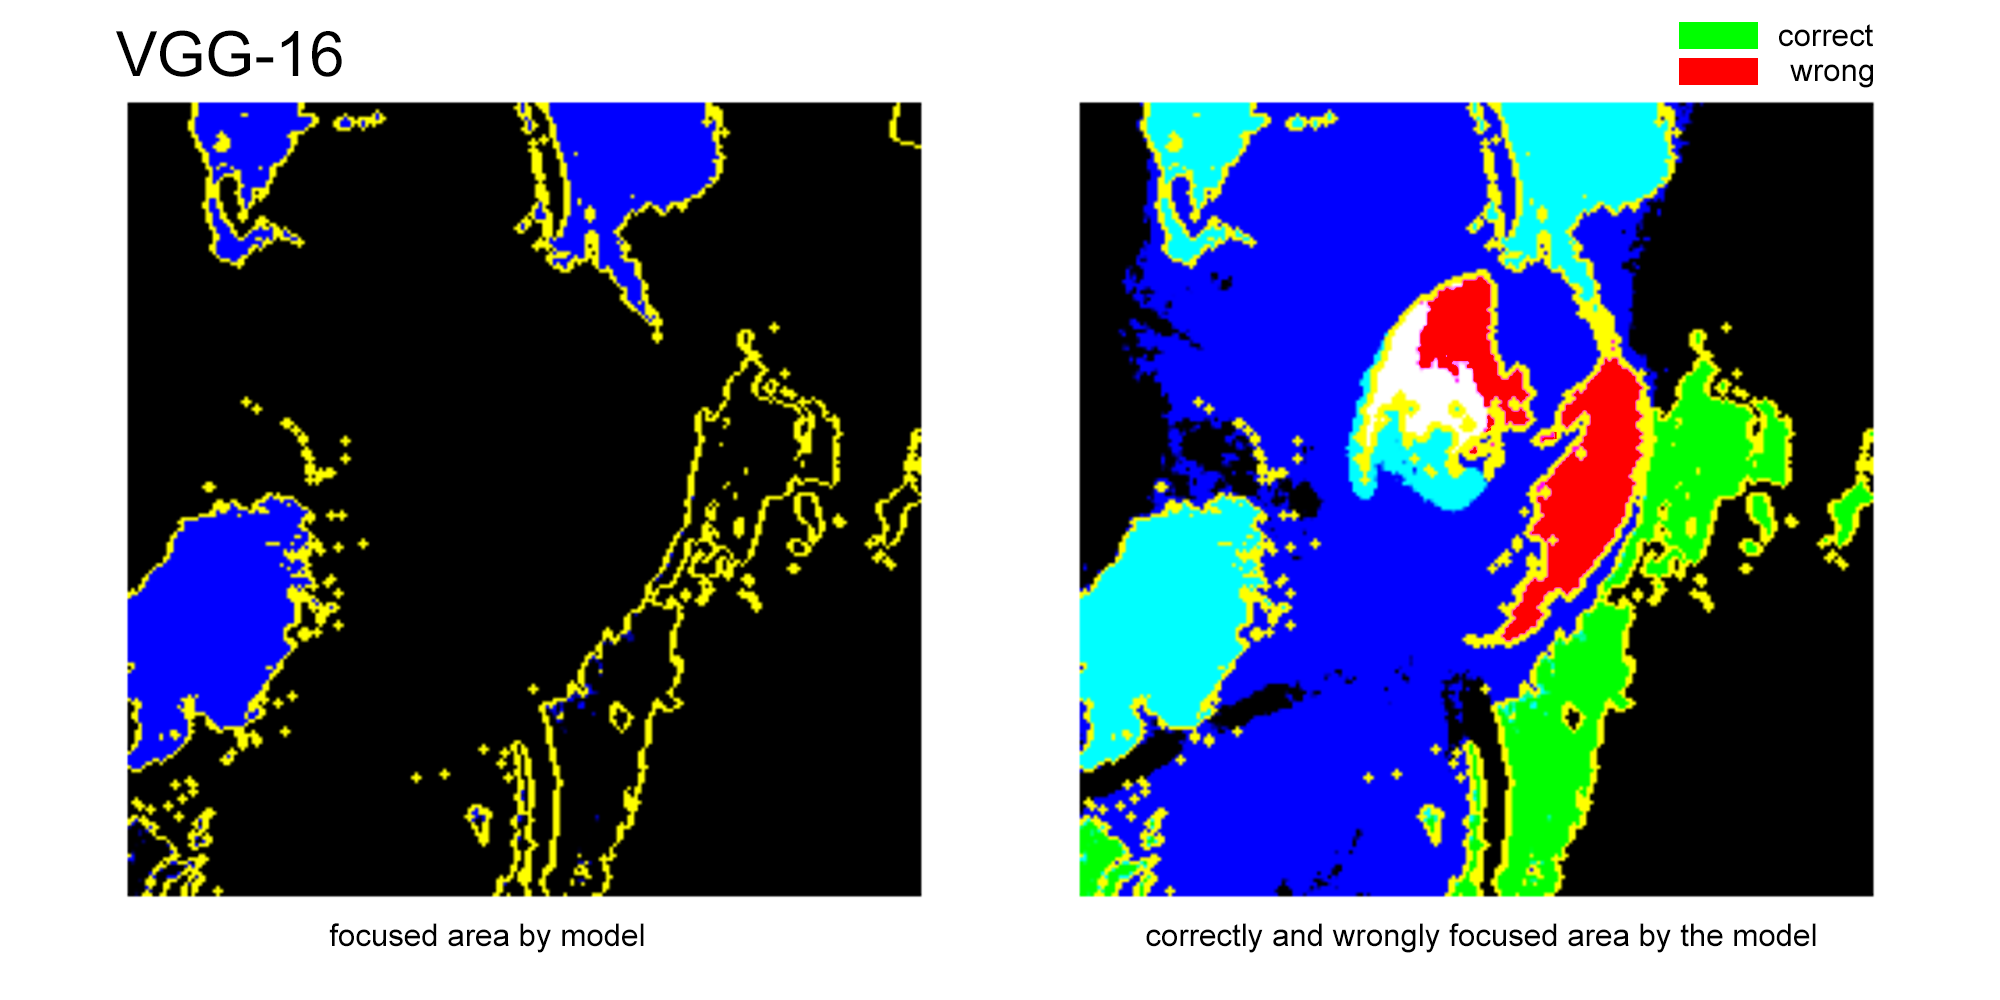
\includegraphics[scale=0.5]{images/fig-47.png}
\caption{Lime Explanation for VGG-16}
\label{fig:x Lime Explanation for VGG-16}
\end{figure}

\newpage
\vspace{5mm}
Given below are the the misclassified image with preprocessing, Superpixels focused area and the model prediction explanation by Lime in VGG-19 -

\vspace{5mm}
\begin{figure}[hbt!]
\centering
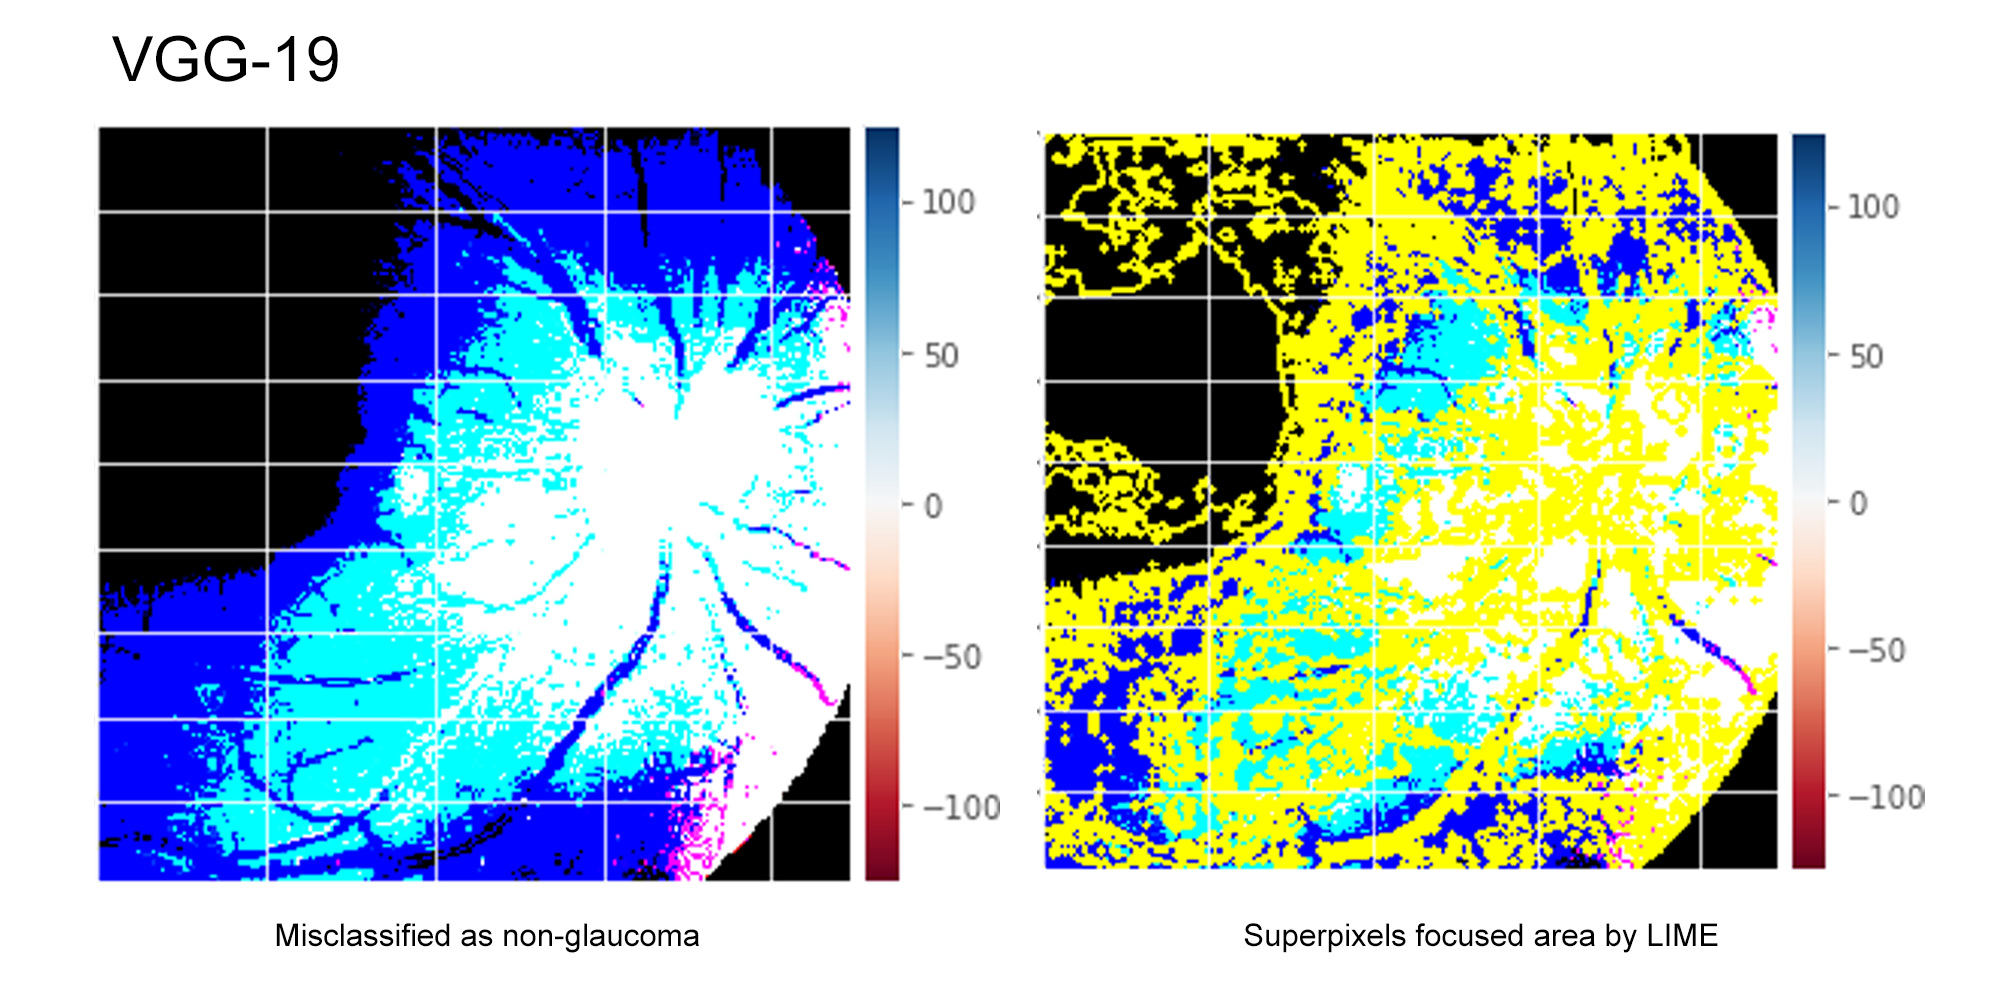
\includegraphics[scale=0.5]{images/fig-48.png}
\caption{Misclassified image with preprocessing and Superpixels focused area by Lime in VGG-19}
\label{fig:x Misclassified image with preprocessing and Superpixels focused area by Lime in VGG-19}
\end{figure}

\vspace{5mm}
\begin{figure}[hbt!]
\centering
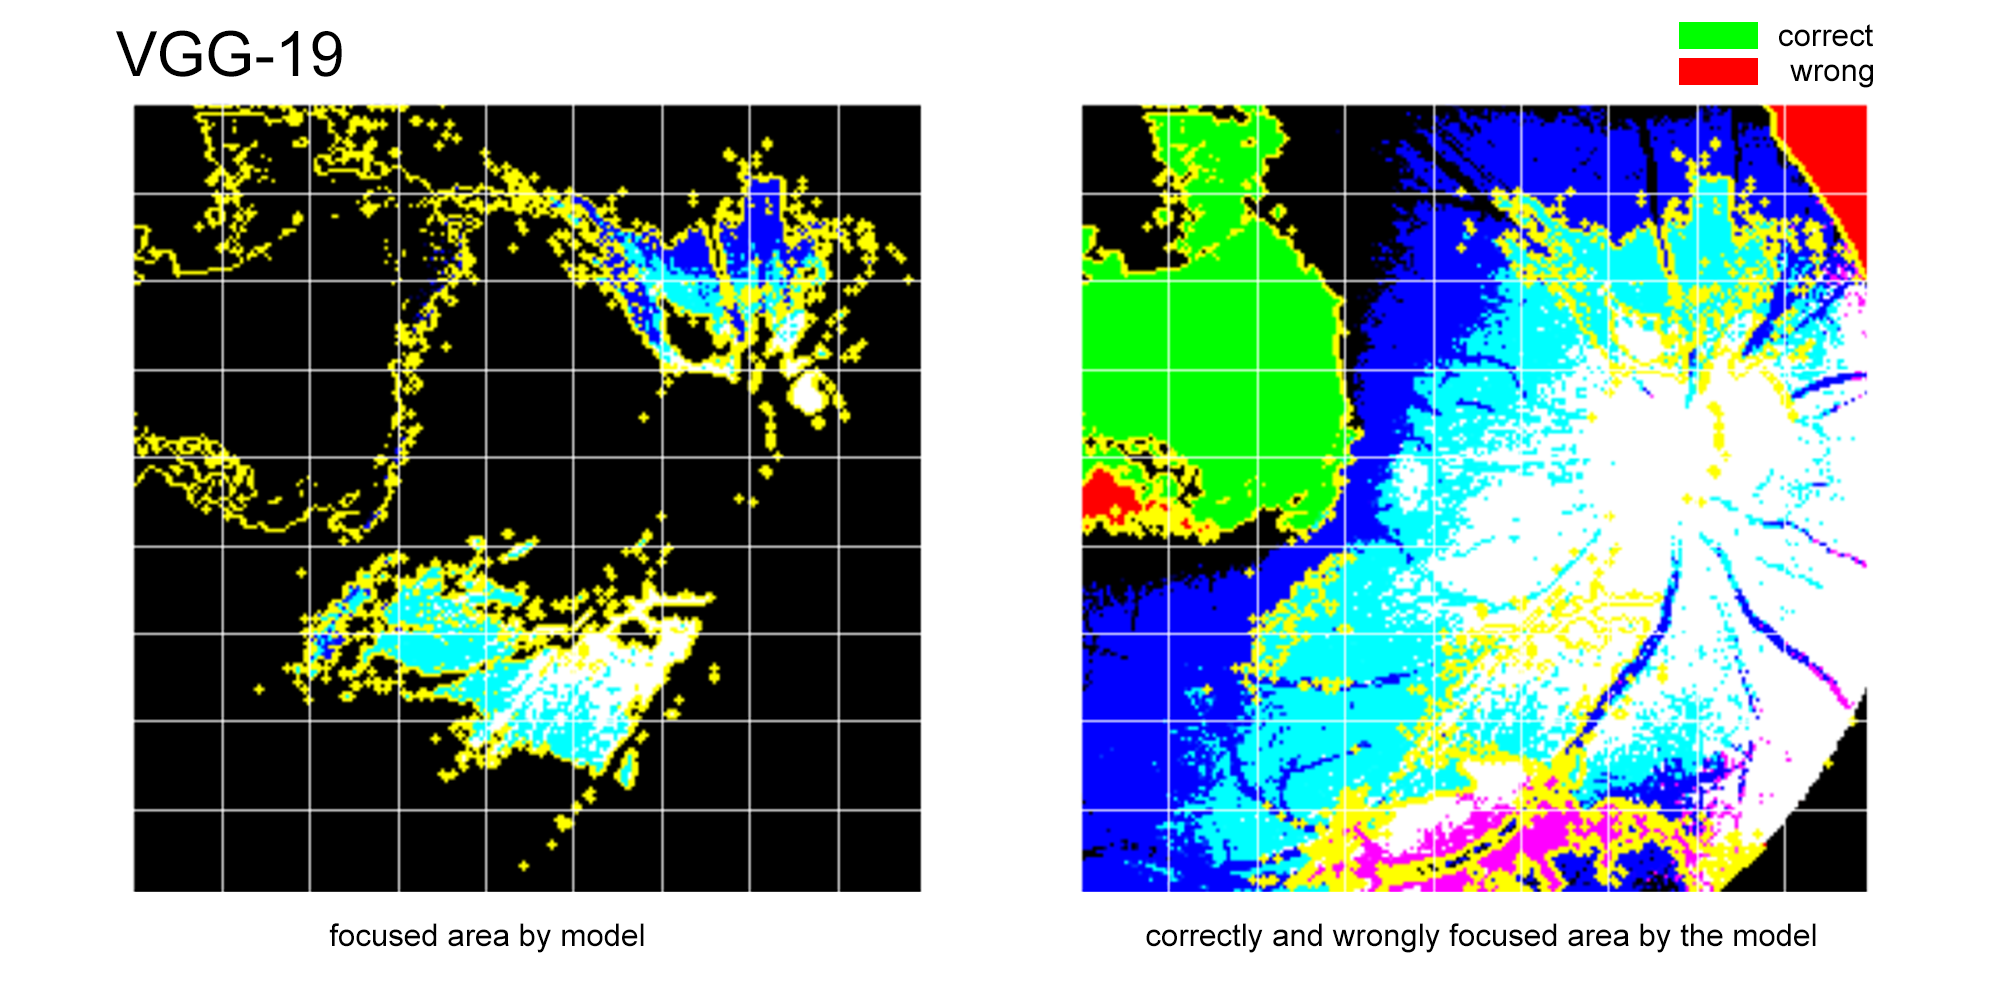
\includegraphics[scale=0.5]{images/fig-49.png}
\caption{Lime Explanation for VGG-19}
\label{fig:x Lime Explanation for VGG-19}
\end{figure}

\newpage
\vspace{5mm}
Given below are the the misclassified image with preprocessing, Superpixels focused area and the model prediction explanation by Lime in ResNet50 -

\vspace{5mm}
\begin{figure}[hbt!]
\centering
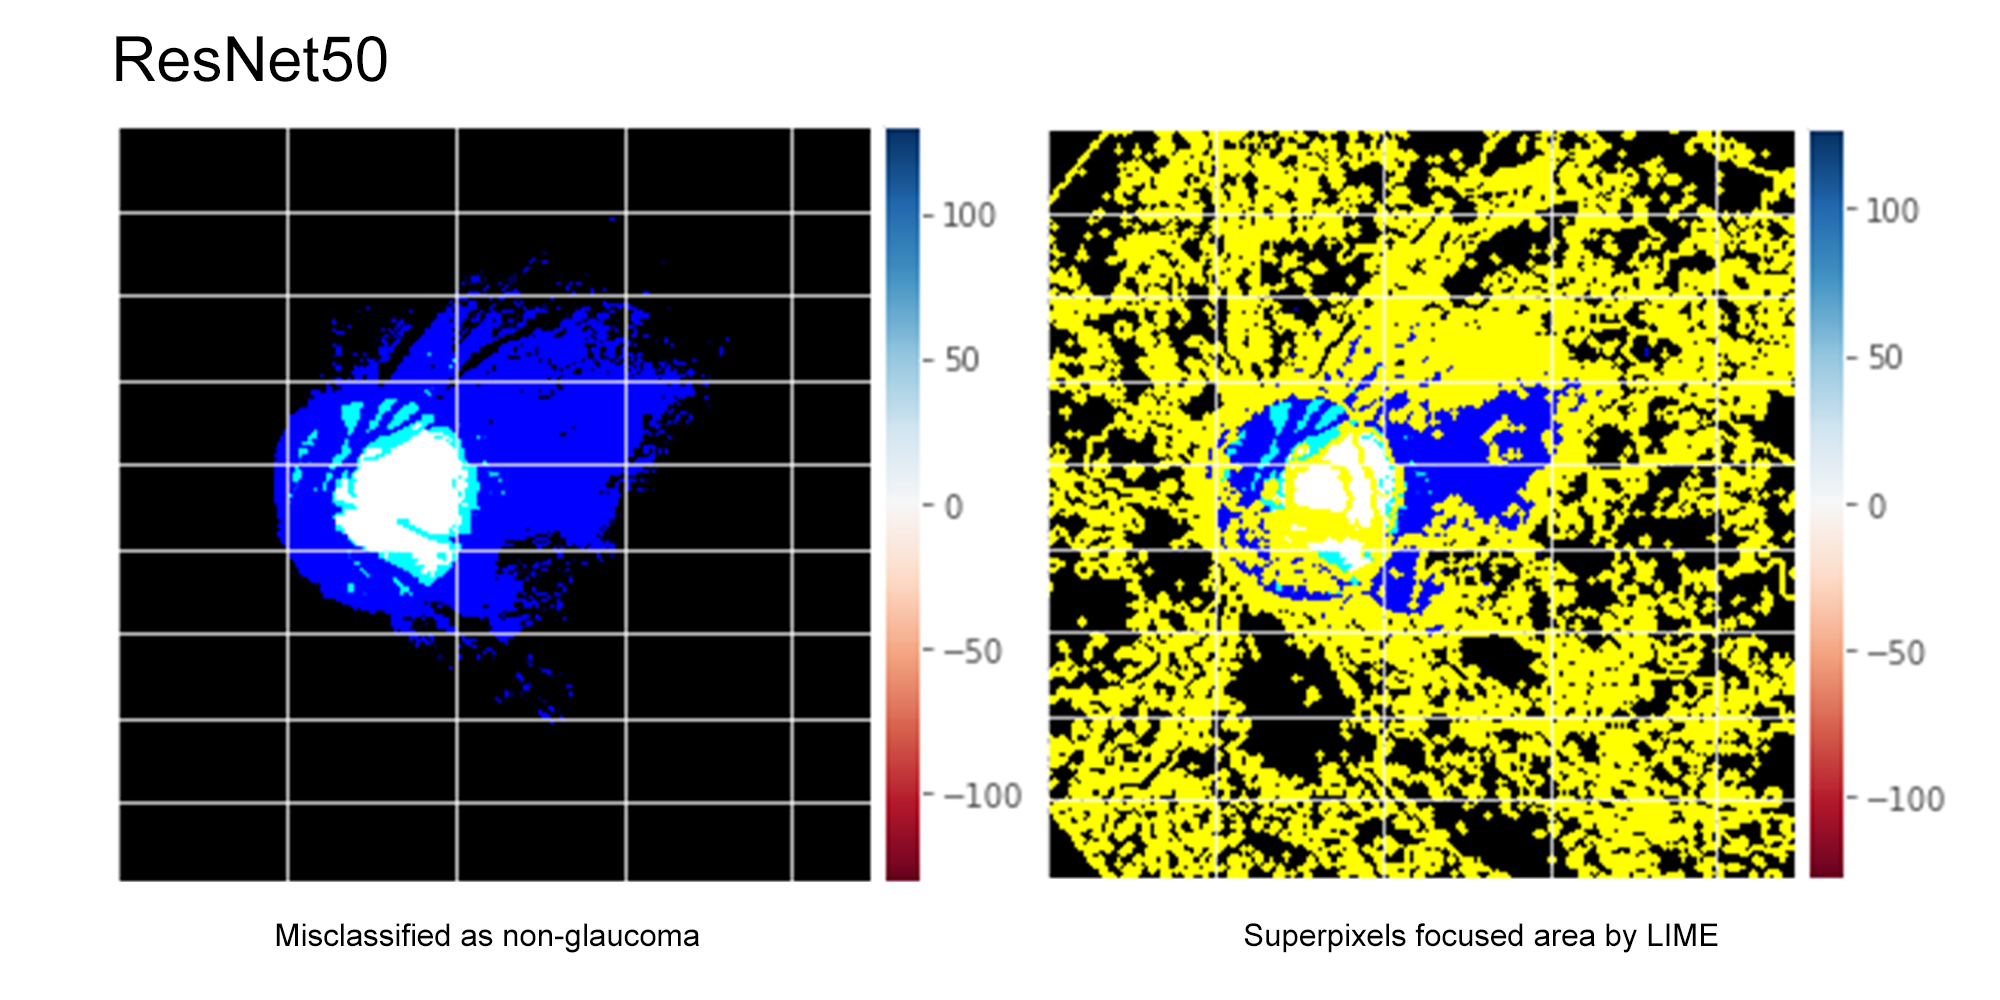
\includegraphics[scale=0.5]{images/fig-50.png}
\caption{Misclassified image with preprocessing and Superpixels focused area by Lime in ResNet50}
\label{fig:x Misclassified image with preprocessing and Superpixels focused area by Lime in ResNet50}
\end{figure}

\vspace{5mm}
\begin{figure}[hbt!]
\centering
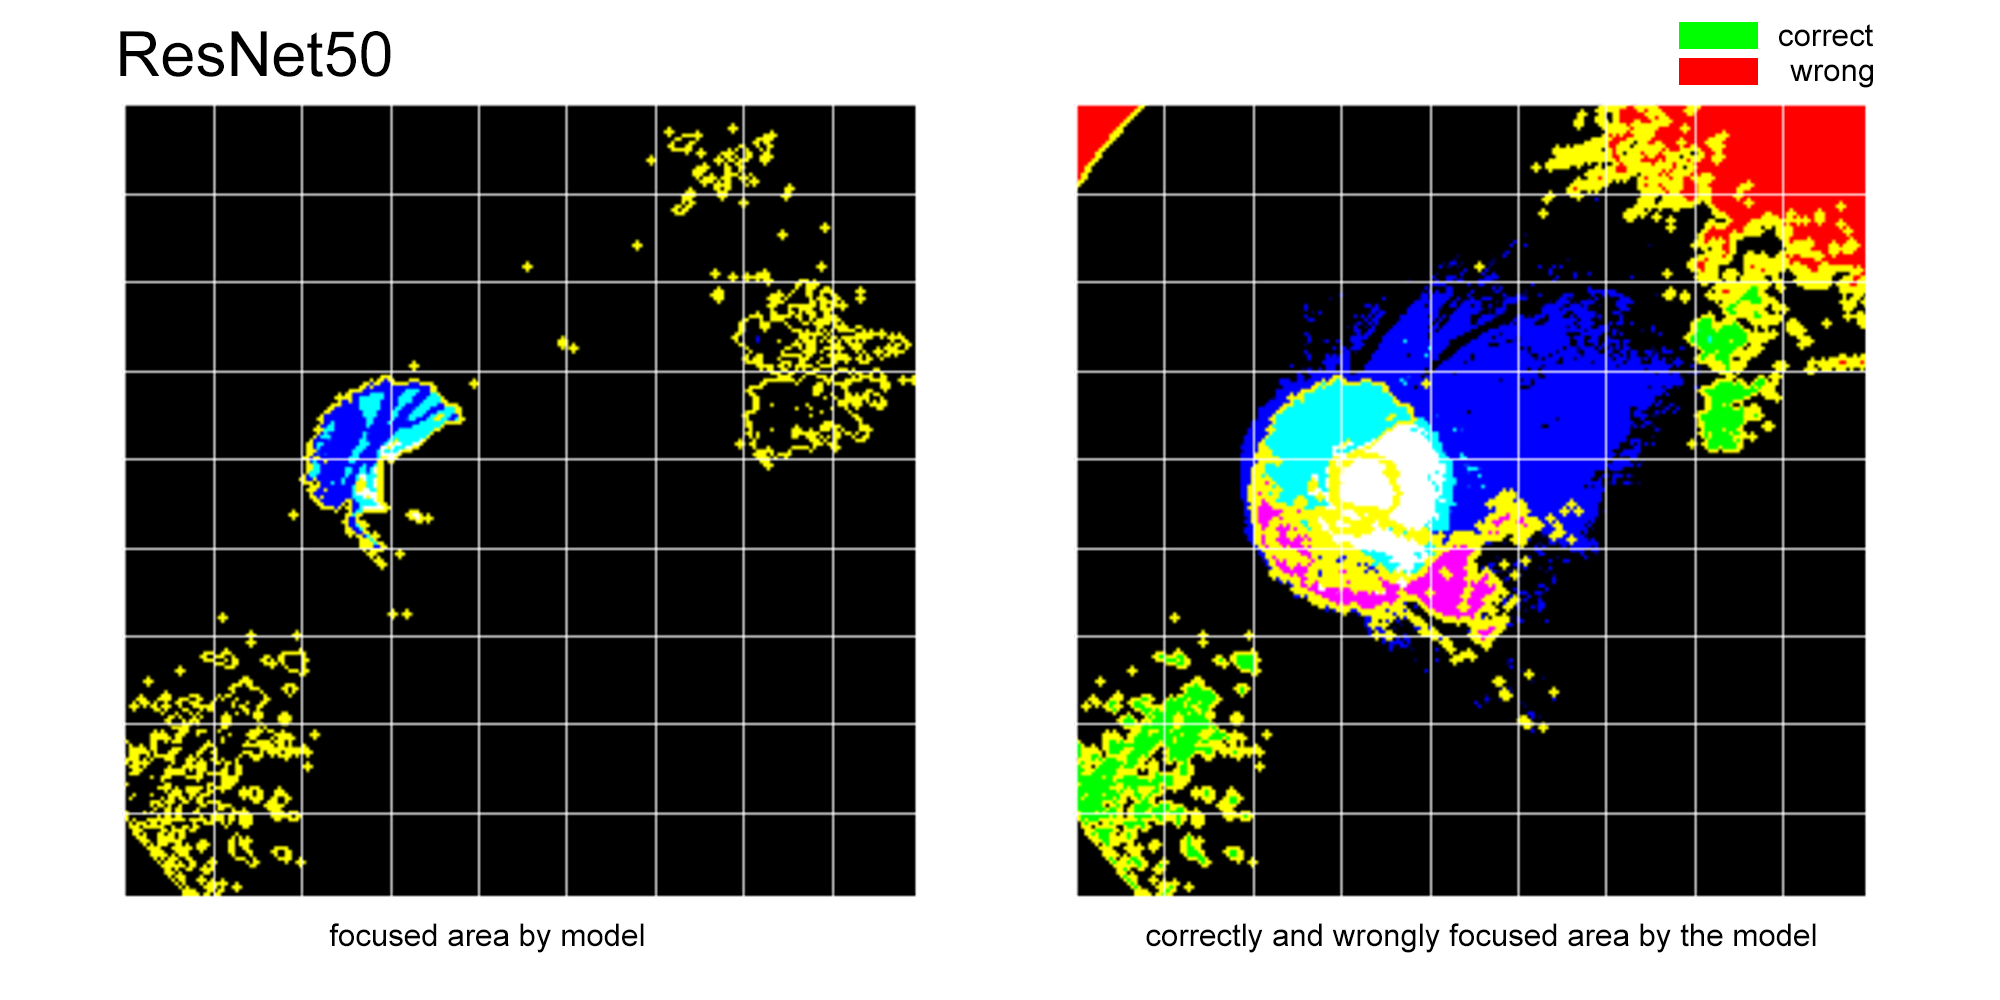
\includegraphics[scale=0.5]{images/fig-51.png}
\caption{Lime Explanation for ResNet50}
\label{fig:x Lime Explanation for ResNet50}
\end{figure}

\newpage
\vspace{5mm}
Now for the single predicted raw fundus image -

\vspace{5mm}
\begin{figure}[hbt!]
\centering
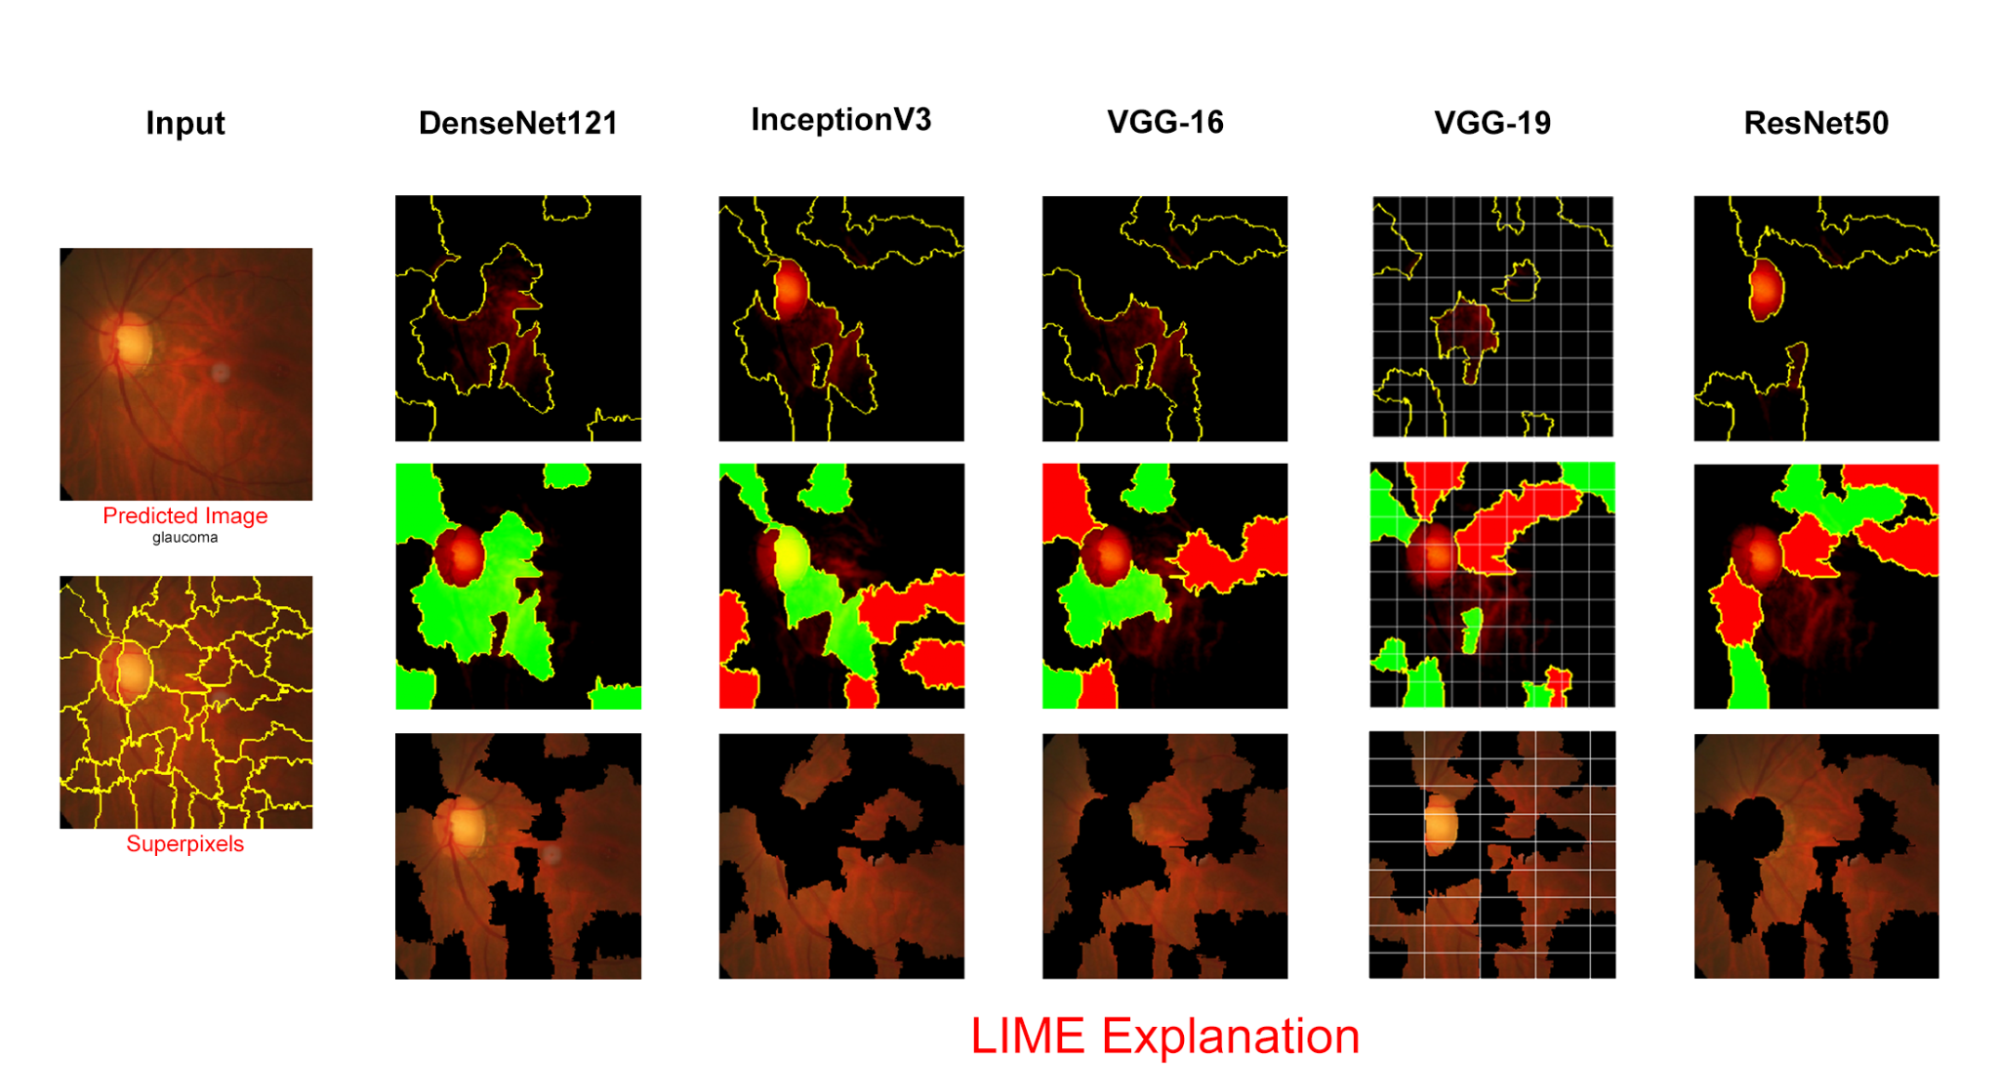
\includegraphics[scale=0.20]{images/fig-52.png}
\caption{Lime Explanation for all models single image predictions}
\label{fig:x Lime Explanation for all models single image predictions}
\end{figure}

\newpage
\section{Result}
These are the single image predictions of all models - 

\textit{( here outputs are given in [n,m] format, where “m” means glaucoma score and “n” means non-glaucoma score )}

\vspace{5mm}
\begin{figure}[hbt!]
\centering
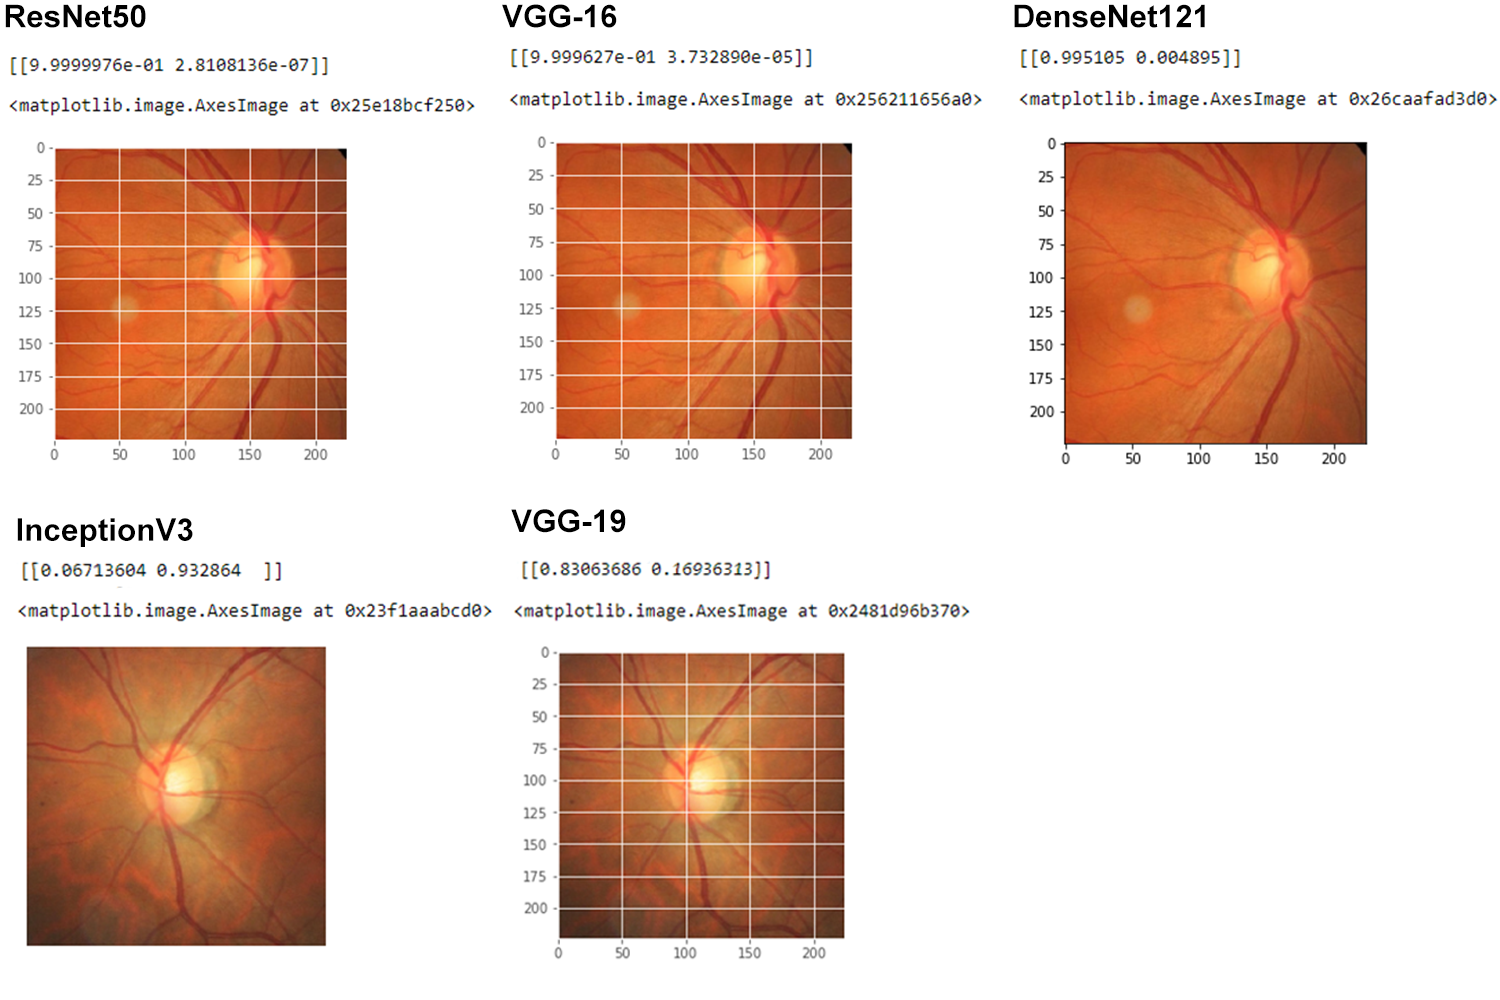
\includegraphics[scale=0.6]{images/fig-53.png}
\caption{Single Image Predictions for all Model}
\label{fig:x Single Image Predictions for all Model}
\end{figure}

\newpage
\vspace{5mm}
\textit{These are batch (50 images/batch) image predictions of all models - ( here [1,0] means glaucoma and [0,1] means non-glaucoma )}


\vspace{5mm}
\begin{figure}[hbt!]
\centering
\includegraphics[scale=0.6]{images/fig-54.png}
\caption{Batch Predictions for DenseNet121}
\label{fig:x Batch Predictions for DenseNet121}
\end{figure}

\vspace{5mm}
\begin{figure}[hbt!]
\centering
\includegraphics[scale=0.6]{images/fig-55.png}
\caption{Batch Predictions for InceptionV3}
\label{fig:x Batch Predictions for InceptionV3}
\end{figure}

\newpage
\vspace{5mm}
\textit{These are batch (50 images/batch) image predictions of all models - ( here [1,0] means glaucoma and [0,1] means non-glaucoma )}

\vspace{5mm}
\begin{figure}[hbt!]
\centering
\includegraphics[scale=0.6]{images/fig-56.png}
\caption{Batch Predictions for VGG-16}
\label{fig:x Batch Predictions for VGG-16}
\end{figure}

\vspace{5mm}
\begin{figure}[hbt!]
\centering
\includegraphics[scale=0.6]{images/fig-57.png}
\caption{Batch Predictions for VGG-19}
\label{fig:x Batch Predictions for VGG-19}
\end{figure}

\vspace{5mm}
\begin{figure}[hbt!]
\centering
\includegraphics[scale=0.6]{images/fig-58.png}
\caption{ Batch Predictions for ResNet50}
\label{fig:x  Batch Predictions for ResNet50}
\end{figure}



\nomenclature{$OOP$}{Object Oriented Programming}